%\documentclass{article}
\documentclass[article, nojss]{jss}
\usepackage{amssymb}
\usepackage{natbib}
\usepackage{graphicx}
\usepackage{color}
\usepackage{verbatim}
\usepackage{hyperref}
\usepackage{url}
\usepackage{listings}

\usepackage{multirow}
\usepackage{multicol}
%\usepackage{enumitem}
%\usepackage[table]{xcolor}
%\usepackage{setspace}
%\usepackage{graphics}
%\usepackage{epsfig}
%\usepackage{indentfirst}
%\usepackage{fancybox}

\usepackage{amsmath}
%\usepackage{rotating}
%\usepackage{booktabs}
%\usepackage[hang,small,bf]{caption}



\setlength{\unitlength}{1cm}
\newcommand{\ex}[1]{\ensuremath{\mathbb{E}[#1]}}
\newcommand{\var}[1]{\ensuremath{\mathrm{Var}[#1]}}
\newcommand{\cov}[1]{\ensuremath{\mathrm{Cov}[#1]}}
\newcommand{\corr}[1]{\ensuremath{\mathrm{Corr}[#1]}}
\newcommand{\bd}[1]{\ensuremath{\mbox{\boldmath $#1$}}}

%\VignetteIndexEntry{Vignette for \textbf{CARBayesST}  package.}


%% almost as usual
\author{Duncan Lee, Alastair Rushworth, Gary Napier and William Pettersson
\\University of Glasgow}
\title{\pkg{CARBayesST} version 3.2: Spatio-Temporal Areal Unit Modelling in \proglang{R} with Conditional Autoregressive Priors}

%% for pretty printing and a nice hypersummary also set:
\Plainauthor{Duncan Lee, Alastair Rushworth, Gary Napier, William Pettersson} %% comma-separated
\Plaintitle{CARBayesST version 3.2: Spatio-Temporal Areal Unit Modelling in R with Conditional Autoregressive Priors} %% without formatting
\Shorttitle{\pkg{CARBayesST}: Spatio-Temporal Areal Unit Modelling} %% a short 


%% an abstract and keywords
\Abstract{
This is a vignette for the \proglang{R} package \pkg{CARBayesST} version 3.2, and is an updated version of a paper in the Journal of Statistical Software in 2018, Volume 84, Issue 9. The package has been developed to model spatio-temporal data relating to a set of non-overlapping areal units that are observed over multiple time periods. These data typically contain spatio-temporal autocorrelation, and this package provides a suite of models for capturing this autocorrelation via random effects that are assigned spatio-temporal extensions of conditional autoregressive (CAR) priors within a hierarchical Bayesian model. \pkg{CARBayesST} is the first dedicated \proglang{R} package for modelling these data in a Bayesian setting using Markov chain Monte carlo (MCMC) simulation. The software can fit a range of models that estimate different aspects of the data, including the estimation of average spatial and temporal trends, and the identification of clusters of areal units that exhibit elevated values. This vignette outlines the class of models that the software can implement, before applying them to exemplar case studies.

}
\Keywords{Bayesian inference, conditional autoregressive priors, spatio-temporal areal unit modelling}
\Plainkeywords{Bayesian inference, conditional autoregressive priors, spatio-temporal areal unit modelling}


 %% without formatting
%% at least one keyword must be supplied

%% publication information
%% NOTE: Typically, this can be left commented and will be filled out by the technical editor
%% \Volume{50}
%% \Issue{9}
%% \Month{June}
%% \Year{2012}
%% \Submitdate{2012-06-04}
%% \Acceptdate{2012-06-04}

%% The address of (at least) one author should be given
%% in the following format:
\Address{
  Duncan Lee\\
  School of Mathematics and Statistics\\ 
  University Place
  University of Glasgow\\
  Glasgow\\ 
  G12 8SQ, Scotland\\
  E-mail: \email{Duncan.Lee@glasgow.ac.uk}\\
  URL: \url{http://www.gla.ac.uk/schools/mathematicsstatistics/staff/duncanlee/}\\
}


\usepackage{Sweave}
\begin{document}
\Sconcordance{concordance:CARBayesST.tex:CARBayesST.Rnw:%
1 84 1 1 0 6 1 1 4 421 1 1 2 1 0 3 1 3 0 1 2 3 1 1 2 13 0 1 2 2 1 1 2 1 %
0 1 3 5 0 1 2 3 1 1 2 1 0 1 1 3 0 1 2 12 1 1 2 1 0 2 1 3 0 1 2 4 1 1 2 %
1 0 1 1 3 0 1 2 2 1 1 2 1 0 1 1 1 7 6 0 1 1 3 0 1 2 12 1 1 2 1 0 3 1 3 %
0 1 2 6 1 1 2 1 0 1 2 1 0 2 1 9 0 1 1 6 0 1 2 2 1 1 2 14 0 1 2 150 1 1 %
2 1 0 4 1 12 0 1 2 3 1 1 2 1 0 1 1 1 5 7 0 1 2 10 1 1 2 1 0 3 1 3 0 1 2 %
2 1 1 2 1 0 1 1 1 2 1 1 1 7 6 0 1 1 3 0 1 2 15 1 1 2 1 0 2 1 3 0 1 2 %
103 1}


%%%%%%%%%%%%%%
%%%% Section 1
%%%%%%%%%%%%%%



\section{Introduction}
Areal unit data are a type of spatial data where the observations relate to a set of $K$ contiguous but non-overlapping areal units, such as electoral wards or census tracts. Each observation relates to an entire areal unit, and thus is typically a summary measure such as an average, proportion, or total, for the entire unit. Examples include the proportion of people who are Catholic in lower super output areas in Northern Ireland (\citealp{lee2015}), the average score on SAT college entrance exams across US states (\citealp{wall2004}), and the total number of cases of chronic obstructive pulmonary disease from populations living in counties in Georgia, USA (\citealp{choiENV11}). Areal unit data have become increasingly available in recent times, due to the creation of databases such as Scottish Statistics (\url{http://statistics.gov.scot/}), and cancer registries such as the Surveillance Epidemiology and End Results programme (\url{http://seer.cancer.gov}). These databases provide data on a set of $K$ areal units for $N$ consecutive time periods, yielding a rectangular array of $K\times N$ spatio-temporal observations. The motivations for modelling these data are varied, and include estimating the effect of a risk factor on a response (see \citealp{wakefield2007}), identifying clusters of contiguous areal units that exhibit an elevated risk of disease compared with neighbouring areas (see \citealp{anderson2014}), and quantifying the level of segregation in a city between two or more different groups (see \citealp{lee2015}). 
 

\hspace{1cm} However, a common challenge when modelling these data is spatio-temporal autocorrelation, whereby observations from geographically close areal units and temporally close time periods tend to have more similar values than units and time periods that are further apart. Temporal autocorrelation occurs because the data relate to largely the same populations in consecutive time periods, while spatial autocorrelation can arise due to unmeasured confounding, neighbourhood effects and grouping effects. A Bayesian inferential approach is typically taken to modelling these data, where the spatio-temporal autocorrelation is modelled via sets of autocorrelated random effects. Conditional autoregressive (CAR, \citealp{besag1991}) priors and spatio-temporal extensions thereof  are typically assigned to these random effects to capture this autocorrelation.  A range of different models have been proposed to date, and the most appropriate model depends on the goals of the analysis.


\hspace{1cm} An array of freely available software can now implement purely spatial areal unit models, including \proglang{BUGS} (\citealp{lunn2009}) and the \proglang{R} packages  \pkg{CARBayes} (\citealp{lee2013}) and \pkg{R-INLA} (\citealp{rue2009}).  However, specialist software for spatio-temporal modelling with conditional autoregressive priors  using MCMC simulation was not previously not available, which has  motivated the development of \pkg{CARBayesST} (\citealp{lee2018}). Section \ref{section2} summarises the models that can be implemented for univariate spatio-temporal data, while Section \ref{section3} summarises the models available for multivariate spatio-temporal data. Section \ref{section4} provides an overview of the software and its functionality. Sections \ref{section5} and \ref{section6} present two worked examples illustrating how to use the software for epidemiological and housing market research, while Section \ref{section7} concludes with a summary of planned future developments.



%%%%%%%%%%%%%%
%%%% Section 2
%%%%%%%%%%%%%%
\section{Spatio-temporal models for univariate areal unit data}\label{section2}
This section outlines the class of univariate models that \pkg{CARBayesST} can implement, and in all cases inference is in a Bayesian setting using Markov chain Monte Carlo (MCMC) simulation. The first part of this section outlines the general hierarchical model that can be fitted, while the second describes the range of space-time random effects structures that are available.


\subsection{General Bayesian hierarchical model}
The study region comprises a set of $k=1,\ldots,K$ non-overlapping areal units $\mathcal{S}=\{\mathcal{S}_{1},\ldots,\mathcal{S}_{K}\}$, and data are recorded for each unit for $t=1,\ldots,N$ consecutive time periods. Thus data are available for a $K\times N$ rectangular array with $K$ rows (spatial units) and $N$ columns (time periods). The response data are denoted by $\mathbf{Y}=(\mathbf{Y}_{1},\ldots,\mathbf{Y}_{N})_{K\times N}$, where $\mathbf{Y}_{t}=(Y_{1t},\ldots,Y_{Kt})$ denotes the $K\times 1$ column vector of observations for all $K$ spatial units for time period $t$. Next, a vector of known offsets is denoted by $\mathbf{O}=(\mathbf{O}_{1},\ldots,\mathbf{O}_{N})_{K\times N}$, where similarly $\mathbf{O}_{t}=(O_{1t},\ldots,O_{Kt})$ denotes the $K\times 1$ column  vector of offsets for time period $t$. Finally, $\mathbf{x}_{kt}=(x_{kt1},\ldots, x_{ktp})$ is a vector of $p$ known covariates for areal unit $k$ and time period $t$, and can include factors or continuous variables and a column of ones for the intercept term. Note, non-linear covariate-response relationships can be included by adding transformations (e.g., squared) or spline basis functions (e.g., using \code{ns()}) of covariates to $\mathbf{x}_{kt}$. \pkg{CARBayesST} can fit the following generalised linear mixed model to these data.

\begin{eqnarray}
Y_{kt}|\mu_{kt}&\sim&f(y_{kt}|\mu_{kt},\nu^{2})~~~~\mbox{for }k=1,\ldots,K,~~t=1,\ldots,N,\label{equation likelihood}\\
g(\mu_{kt})&=&\mathbf{x}_{kt}^{\top}\bd{\beta} + O_{kt} + \psi_{kt},\nonumber\\
\bd{\beta}&\sim&\mbox{N}(\bd{\mu}_{\beta}, \bd{\Sigma}_{\beta}).\nonumber
\end{eqnarray}

The vector of covariate regression parameters are denoted by $\bd{\beta}=(\beta_{1},\ldots,\beta_{p})$, and a multivariate Gaussian prior is assumed with mean $\bd{\mu}_{\beta}$ and diagonal variance matrix $\bd{\Sigma}_{\beta}$  that can be chosen by the user. The $\psi_{kt}$ term is a latent component for areal unit $k$ and time period $t$ encompassing one or more sets of spatio-temporally autocorrelated random effects, and the complete set are denoted by $\bd{\psi}=(\bd{\psi}_{1},\ldots,\bd{\psi}_{N})$, where $\bd{\psi}_{t}=(\psi_{1t},\ldots,\psi_{Kt})$. \pkg{CARBayesST} can fit a number of different spatio-temporal structures for $\psi_{kt}$, which are outlined in Section \ref{section2.2} below. The software can implement Equation \ref{equation likelihood} for binomial, Gaussian and Poisson data models, and the exact specifications of each are given below:

\begin{itemize}
\item \textbf{Binomial} -  $Y_{kt}~\sim~\mbox{Binomial}(n_{kt}, \theta_{kt})$ and $\ln(\theta_{kt}/(1-\theta_{kt}))~=~\mathbf{x}_{kt}^{\top}\bd{\beta} + O_{kt} + \psi_{kt}$. 

\item \textbf{Gaussian} -  $Y_{kt}~\sim~\mbox{N}(\mu_{kt}, \nu^{2})$ and $\mu_{kt}~=~\mathbf{x}_{kt}^{\top}\bd{\beta} + O_{kt} + \psi_{kt}$. 

\item \textbf{Poisson} -  $Y_{kt}~\sim~\mbox{Poisson}(\mu_{kt})$ and $\ln(\mu_{kt})~=~\mathbf{x}_{kt}^{\top}\bd{\beta} + O_{kt} + \psi_{kt}$. 
\end{itemize}

In the binomial model $(n_{kt}, \theta_{kt})$ respectively denote the number of trials and the probability of success in each trial in area $k$ and time period $t$, while in the Gaussian model $\nu^2$ is the observation variance. An inverse-gamma($a,b$) prior is specified for the Gaussian variance $\nu^2$, and default values of $(a=1,~ b=0.01)$  are specified by the software but can be changed by the user.


\subsection{Spatio-temporal random effects models}\label{section2.2}
Spatial autocorrelation is controlled by a symmetric non-negative $K\times K$ neighbourhood or adjacency matrix $\mathbf{W}=(w_{kj})$, where $w_{kj}$ represents the spatial closeness between areal units $(\mathcal{S}_k, \mathcal{S}_j)$. Larger values represent spatial closeness between the two areas in question, where as smaller or zero values correspond to areas that are not spatially close. Most often $\mathbf{W}$ is assumed to be binary, where $w_{kj}=1$ if areal units $(\mathcal{S}_k, \mathcal{S}_j)$ share a common border (i.e., are spatially close) and is zero otherwise. Additionally, $w_{kk}=0$. Under this binary specification the values of $(\psi_{kt}, \psi_{jt})$ for spatially adjacent areal units (where $w_{kj}=1$) are spatially autocorrelated, where as values for non-neighbouring areal units (where $w_{kj}=0$) are conditionally independent given the remaining $\{\psi_{it}\}$ values. This binary specification of $\mathbf{W}$ based on sharing a common border is the most commonly used for areal data, but the only requirement by \pkg{CARBayesST} is for $\mathbf{W}$ to be symmetric, non-negative, and for each row sum to be greater than zero. Similarly, the model \code{ST.CARanova()} defined below uses a binary $N\times N$ temporal neighbourhood matrix $\mathbf{D}=(d_{tj})$, where $d_{tj}=1$ if $|j-t|=1$ and $d_{tj}=0$ otherwise.\\ 

\begin{table}
\begin{tabular}{p{0.22\linewidth}p{0.1\linewidth}p{0.68\linewidth}}
\hline \textbf{Model}&\textbf{Equation}&\textbf{Description}\\\hline
\code{ST.CARlinear()}&(\ref{carlinear})& This model is similar to that proposed by \cite{bernardinelli1995}, and represents the spatio-temporal pattern in the mean response with spatially varying linear time trends. Allowable data models are binomial, Gaussian and Poisson.\\\hline

\code{ST.CARanova()}&(\ref{caranova})& This model is similar to that proposed by \cite{knorrheld2000}, and represents the spatio-temporal pattern in the mean response with an ANOVA style decomposition into overall spatial and temporal main effects and a space-time interaction. Allowable data models are binomial, Gaussian and Poisson. \\\hline

\code{ST.CARsepspatial()}&(\ref{carsepspat})& This model is that proposed by \cite{napier2016}, and represents the spatio-temporal pattern in the mean response with an overall temporal effect and separate independent spatial effects for each time period.  Allowable data models are binomial and Poisson.\\\hline

\code{ST.CARar()}&(\ref{carar})& This model is that proposed by \cite{rushworth2014}, and represents the spatio-temporal pattern in the mean response with a single set of spatially and temporally autocorrelated random effects. The effects follow a multivariate autoregressive process of order 1. Allowable data models are binomial, Gaussian and Poisson.\\\hline

\code{ST.CARadaptive()}&(\ref{caradaptive1})& This model is that proposed by \cite{rushworth2016}, and has the same spatio-temporal random effect structure as the \code{ST.CARar()} model, but with an adaptive spatial autocorrelation structure via estimation of $\mathbf{W}$. Allowable data models are binomial, Gaussian and Poisson.\\\hline

\code{ST.CARlocalised()}&(\ref{carcluster1})& This model is that proposed by \cite{lee2016}, and has the same spatio-temporal random effect structure as the \code{ST.CARar()} model, with an additional piecewise constant intercept term. Allowable data models are binomial and Poisson.\\\hline

\code{ST.CARclustrends()}&(\ref{carclustrends})& This model is that proposed by \cite{napier2018}, and is a mixture model for clustering areas based on their temporal trends in disease risk, where the candidate trend functions have fixed parametric forms or constrained shapes. Allowable data models are binomial and Poisson.\\\hline
\end{tabular}
\caption{Summary of the models available in the \pkg{CARBayesST} package together with the equation numbers defining them mathematically in this vignette.\label{modelsummary}}
\end{table}



\hspace{1cm} \pkg{CARBayesST} can fit the models for $\bd{\psi}$ outlined in Table \ref{modelsummary}, and full details for each one are given below. Out of these models \code{ST.CARlinear()}, \code{ST.CARanova()} and \code{ST.CARar()} are the simplest in terms of parsimony, and thus missing (\code{NA}) values are allowed in the response data ($\mathbf{Y}$) for these models, and are estimated using data augmentation (\citealp{tanner1987}). Missing values are not allowed in the remaining models as they have more complex forms, and exploratory simulated-based testing showed that missing values could not be well recovered in these cases.\\

\code{ST.CARlinear()}\\
This model  is a modification of that proposed by \cite{bernardinelli1995}, and estimates autocorrelated linear time trends for each areal unit. Thus it is  appropriate if the goal of the analysis is to estimate which areas are exhibiting increasing or decreasing (linear) trends in the response over time. The full model specification is given below.

\begin{eqnarray}
\psi_{kt}&=&\beta_{1} + \phi_k + (\alpha + \delta_k)\frac{(t - \bar{t})}{N},\label{carlinear}\\
\phi_k|\bd{\phi}_{-k},\mathbf{W}&\sim&\mbox{N}\left(\frac{\rho_{int}\sum_{j=1}^Kw_{kj}\phi_j}{\rho_{int}\sum_{j=1}^Kw_{kj} + 1-\rho_{int}}, \frac{\tau^2_{int}}{\rho_{int}\sum_{j=1}^Kw_{kj} + 1-\rho_{int}}\right),\nonumber\\
\delta_k|\bd{\delta}_{-k},\mathbf{W}&\sim&\mbox{N}\left(\frac{\rho_{slo}\sum_{j=1}^Kw_{kj}\delta_j}{\rho_{slo}\sum_{j=1}^Kw_{kj} + 1-\rho_{slo}}, \frac{\tau^2_{slo}}{\rho_{slo}\sum_{j=1}^Kw_{kj} + 1-\rho_{slo}}\right),\nonumber\\
\tau^2_{int}, \tau^2_{slo}&\sim&\mbox{Inverse-Gamma}(a,b),\nonumber\\
\rho_{int},\rho_{slo}&\sim&\mbox{Uniform}(0,1),\nonumber\\
\alpha&\sim&\mbox{N}(\mu_{\alpha}, \sigma^2_{\alpha}),\nonumber
\end{eqnarray}

where $\bd{\phi}_{-k}=(\phi_{1},\ldots,\phi_{k-1}, \phi_{k+1},\ldots,\phi_{K})$ and $\bd{\delta}_{-k}=(\delta_{1},\ldots,\delta_{k-1}, \delta_{k+1},\ldots,\delta_{K})$. Here $\bar{t}=(1/N)\sum_{t=1}^N t$, and the linear temporal trend $t^{*}=(t - \bar{t})/N$ runs over a centred unit interval.  Thus areal unit $k$ has its own linear time trend, with a spatially varying intercept $\beta_{1}+\phi_{k}$ and a spatially varying slope $\alpha+\delta_{k}$. Note, the $\beta_1$ term comes from the covariate component $\mathbf{x}_{kt}^{\top}\bd{\beta}$ in (\ref{equation likelihood}). The random effects $\bd{\phi}=(\phi_1,\ldots,\phi_K)$ and  $\bd{\delta}=(\delta_1,\ldots,\delta_K)$ are modelled as spatially autocorrelated by the CAR prior proposed by \cite{leroux2000}, and are mean centred, that is $\sum_{k=1}^{K}\phi_{k}=\sum_{k=1}^{K}\delta_{k}=0$. Here $(\rho_{int}, \rho_{slo})$ are spatial dependence parameters, with values of one corresponding to strong spatial smoothness that is equivalent to the intrinsic CAR prior proposed by  \cite{besag1991}, while values of zero correspond to independence (for example if $\rho_{slo}=0$ then $\delta_k\sim\mbox{N}(0, \tau^2_{slo})$). Flat uniform priors on the unit interval are specified for the spatial dependence parameters $(\rho_{int}, \rho_{slo})$, while conjugate inverse-gamma and Gaussian priors are specified for the random effects variances $(\tau^2_{int}, \tau^2_{slo})$ and the overall slope parameter $\alpha$ respectively. The corresponding hyperparameters $(a, b, \mu_{\alpha}, \sigma^2_{\alpha})$ can be chosen by the user, and the default values are $(a=1, ~b=0.01,~ \mu_{\alpha}=0,~ \sigma^2_{\alpha}=1000)$, which correspond to weakly informative prior distributions. Alternatively, the dependence parameters $(\rho_{int}, \rho_{slo})$ can be fixed at values in the unit interval $[0,1]$ rather than being estimated, by specifying arguments $(\rho_{int}, \rho_{slo})$ in  the \code{ST.CARlinear()} function. Finally, missing (\code{NA}) values are allowed in the response data $\mathbf{Y}$ for this model.\\

\code{ST.CARanova()}\\
The model is a  modification of that proposed by \cite{knorrheld2000},  and decomposes the spatio-temporal variation in the data into 3 components, an overall spatial effect common to all time periods, an overall temporal trend common to all spatial units, and a set of independent space-time interactions. This model is appropriate if the goal is to estimate overall time trends and spatial patterns, and the model  is given by.

\begin{eqnarray}
\psi_{kt}&=&\phi_k +  \delta_t   + \gamma_{kt},\label{caranova}\\
\phi_k|\bd{\phi}_{-k},\mathbf{W}&\sim&\mbox{N}\left(\frac{\rho_{S}\sum_{j=1}^Kw_{kj}\phi_j}{\rho_{S}\sum_{j=1}^Kw_{kj} + 1-\rho_{S}}, \frac{\tau^2_{S}}{\rho_{S}\sum_{j=1}^Kw_{kj} + 1-\rho_{S}}\right),\nonumber\\
\delta_t|\bd{\delta}_{-t},\mathbf{D}&\sim&\mbox{N}\left(\frac{\rho_{T}\sum_{j=1}^N d_{tj}\delta_j}{\rho_{T}\sum_{j=1}^N d_{tj} + 1-\rho_{T}}, \frac{\tau^2_{T}}{\rho_{T}\sum_{j=1}^N d_{tj}+1-\rho_{T}}\right),\nonumber\\
\gamma_{kt}&\sim&\mbox{N}(0, \tau^2_{I} ),\nonumber\\
\tau^2_{S}, \tau^2_{T}, \tau^2_{I}&\sim&\mbox{Inverse-Gamma}(a,b),\nonumber\\
\rho_{S},\rho_{T}&\sim&\mbox{Uniform}(0,1).\nonumber
\end{eqnarray}


Here the spatio-temporal autocorrelation is modelled by a common set of spatial random effects $\bd{\phi}=(\phi_1,\ldots,\phi_K)$ and a common set of temporal random effects  $\bd{\delta}=(\delta_1,\ldots,\delta_N)$, and both are modelled by the CAR prior proposed by \cite{leroux2000}. Additionally, the model can incorporate an optional set of independent space-time interactions $\bd{\gamma}=(\gamma_{11},\ldots,\gamma_{KN})$, which can be specified by the argument \code{interaction=TRUE} (the default) in the function call. All sets of random effects are mean centred. Fixed uniform $(\rho_{S},\rho_{T})$  and conjugate $(\tau^2_{S}, \tau^2_{T}, \tau^2_{I})$ priors are specified for the remaining parameters, and the default specifications for the latter are $(a=1,~ b=0.01)$. Alternatively, the  dependence parameters $(\rho_{S}, \rho_{T})$ can be fixed at values in the unit interval $[0,1]$ rather than being estimated in the model, for full details see the help file for this function. Finally, missing (\code{NA}) values are allowed in the response data $\mathbf{Y}$ for this model.\\


\code{ST.CARsepspatial()}\\
The model is a generalisation of that proposed by \cite{napier2016}, and represents the data by two components,  an overall temporal trend, and separate spatial surfaces for each time period that share a common spatial dependence parameter but have different spatial variances. This model is appropriate if the goal is to estimate both a common overall temporal trend and the extent to which the spatial variation in the response has changed over time. The model specification is given below.


\begin{eqnarray}
\psi_{kt}&=&\phi_{kt} +  \delta_t,\label{carsepspat}\\
\phi_{kt}|\bd{\phi}_{-kt},\mathbf{W}&\sim&\mbox{N}\left(\frac{\rho_{S}\sum_{j=1}^Kw_{kj}\phi_{jt}}{\rho_{S}\sum_{j=1}^Kw_{kj} + 1-\rho_{S}}, \frac{\tau^2_{t}}{\rho_{S}\sum_{j=1}^Kw_{kj} + 1-\rho_{S}}\right),\nonumber\\
\delta_t|\bd{\delta}_{-t},\mathbf{D}&\sim&\mbox{N}\left(\frac{\rho_{T}\sum_{j=1}^N d_{tj}\delta_j}{\rho_{T}\sum_{j=1}^N d_{tj} + 1-\rho_{T}}, \frac{\tau^2_{T}}{\rho_{T}\sum_{j=1}^N d_{tj}+1-\rho_{T}}\right),\nonumber\\
\tau^2_{1},\ldots, \tau^2_{N}, \tau^2_{T}, &\sim&\mbox{Inverse-Gamma}(a,b),\nonumber\\
\rho_{S}, \rho_{T}&\sim&\mbox{Uniform}(0,1),\nonumber
\end{eqnarray}

where $\bd{\phi}_{-k,t}=(\phi_{1,t},\ldots,\phi_{k-1,t}, \phi_{k+1,t},\ldots,\phi_{K,t})$. This model fits an overall temporal trend to the data $\bd{\delta}=(\delta_1,\ldots,\delta_{N})$ that is common to all areal units, which is augmented with a separate (uncorrelated) spatial surface $\bd{\phi}_t=(\phi_{1t},\ldots, \phi_{Kt})$ at each time period $t$. The overall temporal trend and each spatial surface are modelled by the CAR prior proposed by \cite{leroux2000}, and the latter have a common spatial dependence parameter $\rho_S$ but a temporally-varying variance parameter $\tau^2_{t}$. Thus the collection $(\tau^2_{1},\ldots, \tau^2_{N})$ allows one to examine the extent to which the magnitude of the spatial variation in the data has changed over time. Note that here we fix $\rho_S$ to be constant in time as it is not orthogonal to $\tau^{2}_t$, thus if it varied then any changes in $\tau^{2}_t$ would not directly correspond to changes in spatial variance over time. As with all other models the random effects are zero-mean centred, while flat and conjugate priors are specified for $(\rho_S, \rho_T)$ and $(\tau^2_{T}, \tau^2_{1},\ldots, \tau^2_{N})$ respectively. Alternatively, the  dependence parameters $(\rho_{S}, \rho_{T})$ can be fixed at values in the unit interval $[0,1]$ rather than being estimated in the model. Missing (\code{NA}) values are not allowed in the response data $\mathbf{Y}$ in this model.\\




\code{ST.CARar()}\\
There are two versions of this model, which are based on either a first (AR(1)) or a second (AR(2)) order temporal autoregressive process. The first order model is that proposed by \cite{rushworth2014}, and represents the spatio-temporal structure with a multivariate first order autoregressive process with a spatially autocorrelated precision matrix. The second model extends this by using a multivariate second order autoregressive process with a spatially autocorrelated precision matrix. These models are appropriate if one wishes to estimate the  evolution of the spatial random effects surface over time. The model specifications in both cases are given below.\vspace{0.5cm}


\textbf{AR(1) model}


\begin{eqnarray}
\psi_{kt}&=&\phi_{kt},\label{carar}\\
\bd{\phi}_t|\bd{\phi}_{t-1} & \sim & \mbox{N}\left(\rho_T\bd{\phi}_{t-1}, \tau^{2} \mathbf{Q}(\mathbf{W},\rho_S)^{-1}\right)\hspace{1cm} t=2,\ldots,N,\nonumber\\
\bd{\phi}_1 & \sim & \mbox{N}\left(\mathbf{0}, \tau^{2} \mathbf{Q}(\mathbf{W},\rho_S)^{-1}\right),\nonumber\\
\tau^2&\sim&\mbox{Inverse-Gamma}(a,b),\nonumber\\
\rho_S,\rho_T&\sim&\mbox{Uniform}(0,1).\nonumber
\end{eqnarray}


\textbf{AR(2) model}


\begin{eqnarray}
\psi_{kt}&=&\phi_{kt},\label{carar2}\\
\bd{\phi}_t|\bd{\phi}_{t-1}, \bd{\phi}_{t-2} & \sim & \mbox{N}\left(\rho_{T_1}\bd{\phi}_{t-1}+\rho_{T_2}\bd{\phi}_{t-2}, \tau^{2} \mathbf{Q}(\mathbf{W},\rho_S)^{-1}\right)\hspace{1cm} t=3,\ldots,N,\nonumber\\
\bd{\phi}_1, \bd{\phi}_2 & \sim & \mbox{N}\left(\mathbf{0}, \tau^{2} \mathbf{Q}(\mathbf{W},\rho_S)^{-1}\right),\nonumber\\
\tau^2&\sim&\mbox{Inverse-Gamma}(a,b),\nonumber\\
\rho_S&\sim&\mbox{Uniform}(0,1),\nonumber\\
f(\rho_{T_1}, \rho_{T_2}) &\propto&1.\nonumber
\end{eqnarray}


Here $\bd{\phi}_{t}=(\phi_{1t},\ldots,\phi_{Kt})$ is the vector of random effects for time period $t$, which  evolve over time via a multivariate first or second order autoregressive process with temporal autoregressive parameter $\rho_T$ (AR(1) model) or $(\rho_{T_1}, \rho_{T_2})$ (AR(2) model). The choice between these two options is made by the argument \code{AR=1}  or \code{AR=2} within the function. Thus temporal autocorrelation is induced via the mean  while spatial autocorrelation is induced by the variance $\tau^{2} \mathbf{Q}(\mathbf{W},\rho_S)^{-1}$. The corresponding precision matrix $\mathbf{Q}(\mathbf{W},\rho_S)$ was proposed by \cite{leroux2000} and corresponds to the CAR models used in the other models above. The algebraic form of this matrix is given by

\begin{equation}
\mathbf{Q}(\mathbf{W},\rho_S)=\rho_S[\mbox{diag}(\mathbf{W}\mathbf{1}) - \mathbf{W}] + (1-\rho_S)\mathbf{I},\label{Lerouxjoint}
\end{equation}

where $\mathbf{1}$ is the $K\times 1$ vector of ones while $\mathbf{I}$ is the $K\times K$ identity matrix. In common with all other models the random effects are zero-mean centred, while flat and conjugate inverse-gamma priors are specified for $(\rho_S, \rho_T, \rho_{T_1}, \rho_{T_2})$ and $\tau^2$ respectively, with $(a=1, b=0.01)$ being the default hyperparameter values for the latter. The  dependence parameters $(\rho_{S}, \rho_{T})$ can be fixed at values in the unit interval $[0,1]$ rather than being estimated in the model, while $(\rho_{T_1}, \rho_{T_2})$ can also be fixed if required. Finally, missing (\code{NA}) values are allowed in the response data $\mathbf{Y}$ for this model.\vspace{1cm}


\code{ST.CARadaptive()}\\
The model is that proposed by \cite{rushworth2016}, and is an extension of \code{ST.CARar()} proposed by \cite{rushworth2014} to allow for spatially adaptive smoothing. It is appropriate if one believes that the residual spatial autocorrelation in the response after accounting for the covariates is consistent over time but has a localised structure. That is, it is strong in some parts of the study region but weak in others. The model has the same autoregressive random effects structure as the first order  \code{ST.CARar()} model, namely:

\begin{eqnarray}
\psi_{kt}&=&\phi_{kt},\label{caradaptive1}\\
\bd{\phi}_t|\bd{\phi}_{t-1} & \sim & \mbox{N}\left(\rho_T\bd{\phi}_{t-1}, \tau^{2} \mathbf{Q}(\mathbf{W},\rho_S)^{-1}\right)\hspace{1cm} t=2,\ldots,N,\nonumber\\
\bd{\phi}_1 & \sim & \mbox{N}\left(\mathbf{0}, \tau^{2} \mathbf{Q}(\mathbf{W},\rho_S)^{-1}\right),\nonumber\\
\tau^2&\sim&\mbox{Inverse-Gamma}(a,b),\nonumber\\
\rho_S,\rho_T&\sim&\mbox{Uniform}(0,1).\nonumber
\end{eqnarray}


However, the random effects from  \code{ST.CARar()} have a single level of spatial dependence that is controlled by $\rho_S$. All pairs of adjacent areal units (for which $w_{kj}=1$) will have strongly autocorrelated random effects if $\rho_S$ is close to one, while no such spatial dependence will exist anywhere if $\rho_S$ is close to zero. However, real data may exhibit spatially varying dependencies, as two adjacent areal units may exhibit similar values suggesting a value of $\rho_S$ close to one, while another adjacent pair may exhibit very different values suggesting a value of $\rho_S$ close to zero.

\hspace{1cm} This model allows for localised spatial autocorrelation by allowing spatially neighbouring  random effects to be correlated (inducing smoothness) or conditionally independent (no smoothing), which is  achieved by modelling the non-zero elements of the neighbourhood matrix $\mathbf{W}$  as unknown parameters, rather than assuming they are fixed at 1. For this model $\mathbf{W}$ must be a binary matrix. These adjacency parameters are collectively denoted by $\mathbf{w}^{+}=\{w_{kj}|k\sim j\}$, where $k\sim j$ means areas $(k,j)$ are neighbours and $w_{kj}=1$. Estimating $w_{kj}\in\mathbf{w}^{+}$ equal to zero means $(\phi_{kt}, \phi_{jt})$  are conditionally independent for all time periods $t$  given the remaining random effects, while estimating it close to one means they are correlated. These adjacency parameters in $\mathbf{w}^{+}$ are each modelled on the unit interval, by assuming a multivariate Gaussian prior distribution on the transformed scale $\mathbf{v}^+ = \log\left(\mathbf{w}^{+}/(\mathbf{1} - \mathbf{w}^{+}) \right)$.  This prior is a shrinkage model with a constant mean $\mu$ and a diagonal variance matrix with variance parameter $\zeta^2$, and is given by


\begin{eqnarray}
f(\mathbf{v}^{+}|\tau^2_w, \mu) & \propto & \exp\left[-\frac{1}{2\tau^2_w}\left(\sum_{v_{ik}\in\mathbf{v}^{+}}(v_{ik} - \mu)^2\right)\right], \label{caradaptive2}\\
\tau^{2}_w&\sim&\mbox{Inverse-Gamma}(a, b).\nonumber
\end{eqnarray}

The prior distribution for $\mathbf{v}^+$ assumes that the degree of smoothing between pairs of adjacent random effects is not spatially dependent, which results from the  work of \cite{rushworth2016}. Under small values of $\tau_w^2$ the elements of  $\mathbf{v}^+$ are shrunk to $\mu$, and here we follow the work of \cite{rushworth2016} and fix $\mu=15$ because it avoids numerical issues when transforming between $\mathbf{v}^+$ and $\mathbf{w}^+$ and implies a prior preference for values of $w_{kj}$ close to 1.  That is as $\tau^2_w \rightarrow 0$ the prior becomes the global smoothing model \code{ST.CARar()}, where as when $\tau^{2}_{w}$ increases both small and large values in $\mathbf{w}^{+}$ are supported by the prior. As with the other models the default values for the inverse-gamma prior for $\tau_w^2$ are $(a=1, b=0.01)$. It is possible to fix $\rho_S$ using the \code{rho} argument. For further details see \cite{rushworth2016}. Missing (\code{NA}) values are not allowed in the response data $\mathbf{Y}$ in this model.\\


\code{ST.CARlocalised()}\\
The model was proposed by \cite{lee2016}, and augments the smooth spatio-temporal variation in \code{ST.CARar()} with a piecewise constant intercept process.  This model is appropriate when the aim of the analysis is to identify clusters of areas that exhibit elevated (or reduced) values of the response compared with their geographical and temporal neighbours. This model captures any step-changes in the response via the mean function, and is given by


\begin{eqnarray}
\psi_{kt}&=&\lambda_{Z_{kt}} + \phi_{kt},\label{carcluster1}\\
\bd{\phi}_t|\bd{\phi}_{t-1} & \sim & \mbox{N}\left(\rho_T\bd{\phi}_{t-1}, \tau^{2} \mathbf{Q}(\mathbf{W})^{-}\right)\hspace{1cm} t=2,\ldots,N,\nonumber\\
\bd{\phi}_1 & \sim & \mbox{N}\left(\mathbf{0}, \tau^{2} \mathbf{Q}(\mathbf{W})^{-}\right),\nonumber\\
\tau^2&\sim&\mbox{Inverse-Gamma}(a,b),\nonumber\\
\rho_T&\sim&\mbox{Uniform}(0,1),\nonumber
\end{eqnarray}

where the `$^{-}$' in $\mathbf{Q}(\mathbf{W})^{-}$ denotes a generalised inverse. The random effects $\bd{\phi}=(\bd{\phi}_{1},\ldots,\bd{\phi}_{T})$ are modelled by a simplification of the \code{ST.CARar()} model with a first order autoregressive process where $\rho_S=1$, which corresponds to the intrinsic CAR model proposed by \cite{besag1991}. Note, for this model the inverse $\mathbf{Q}(\mathbf{W})^{-1}$ does not exist as the precision matrix is singular. This simplification is made so that the random effects $\bd{\phi}$ capture the globally smooth spatio-temporal autocorrelation in the data, allowing the other component $\lambda_{Z_{kt}}$ to capture localised clustering and step-changes. This second component is a piecewise constant clustering or intercept process $\lambda_{Z_{kt}}$. Spatially and  temporally adjacent data points $(Y_{kt}, Y_{js})$ will be similar if they have the same intercept, that is if $\lambda_{Z_{kt}}=\lambda_{Z_{js}}$, but exhibit a step-change if they are have different intercepts, that is if $\lambda_{Z_{kt}}\neq\lambda_{Z_{js}}$. The piecewise constant intercept or clustering process  comprises at most $G$ distinct levels, making this component a piecewise constant intercept term. The $G$ levels are ordered via the prior specification:

\begin{eqnarray}
\lambda_{j}&\sim&\mbox{Uniform}(\lambda_{j-1},\lambda_{j+1})~~~~\mbox{for }j=1,\dots,G,\label{carcluster2}
\end{eqnarray}

where $\lambda_{0}=-\infty$ and  $\lambda_{G+1}=\infty$. Here $Z_{kt}\in\{1,\ldots,G\}$ and controls the assignment of the $(k,t)$th data point to one of the $G$ intercept levels. A penalty based approach is used to model $Z_{kt}$, where $G$ is chosen larger than necessary and a penalty prior is used  to shrink it to the middle intercept level.  This middle level is $G^{*}=(G+1)/2$ if $G$ is odd and $G^{*}=G/2$ if $G$ is even, and this penalty ensures that $Z_{kt}$ is only in the extreme low and high risk classes if supported by the data. Thus $G$ is the maximum number of distinct intercept terms allowed in the model, and is not the actual number of intercept terms estimated in the model. The allocation prior is independent across areal units but correlated in time, and is given by:


\begin{eqnarray}
f(Z_{kt}|Z_{k,t-1})&=&\frac{\exp(-\delta[(Z_{kt}-Z_{k,t-1})^{2} +(Z_{kt}-G^{*})^{2}])}{\sum_{r=1}^{G}\exp(-\delta[(r-Z_{k,t-1})^{2}+(r-G^{*})^{2}])}~~~~\mbox{for } t=2,\ldots,N,\label{carcluster3}\\
f(Z_{k1})&=&\frac{\exp(-\delta(Z_{k1}-G^{*})^{2})}{\sum_{r=1}^{G}\exp(-\delta(r-G^{*})^{2})},\nonumber\\
\delta&\sim&\mbox{Uniform}(1,m).\nonumber
\end{eqnarray}

Temporal autocorrelation is induced by the $(Z_{kt}-Z_{k,t-1})^{2}$ component of the penalty, while the $(Z_{kt}-G^{*})^{2}$ component penalises class indicators $Z_{kt}$ towards the middle risk class $G^{*}$. The size of this penalty and hence the amount of smoothing that is imparted on $\mathbf{Z}$ is controlled by $\delta$, which is assigned a uniform prior. The default value is $m=10$, and full details of this model can be found in \cite{lee2016}. Missing (\code{NA}) values are not allowed in the response data $\mathbf{Y}$ in this model.\\

\textbf{ST.CARclustrends()}\\
The model is that proposed by \cite{napier2018} and represents the data by two components, an overall spatial pattern, and  a mixture of temporal trend functions with fixed parametric forms (e.g.\ linear, step-change) or constrained shapes (e.g.\ monotonically increasing). Note here that due to identifiability issues, covariates are not allowed in this model, but offsets (using the \code{offset()} function) are allowed. This model is appropriate if the goal is to identify clusters of areas that exhibit similar temporal trends. The model specification is given below.

\begin{eqnarray}
\psi_{kt} &=& \phi_k +  \sum_{s=1}^S   \omega_{ks} f_s(t|\bd{\gamma}_s),\label{carclustrends}\\
\phi_k|\bd{\phi}_{-k},\mathbf{W},\rho, \tau^2&\sim&\mbox{N}\left(\frac{\rho\sum_{j=1}^K w_{kj}\phi_j}{\rho\sum_{j=1}^Kw_{kj} + 1-\rho}, \frac{\tau^2}{\rho\sum_{j=1}^K w_{kj} + 1-\rho}\right),\nonumber\\
\tau^2 &\sim&\mbox{Inverse-Gamma}(a,b),\nonumber\\
\rho&\sim&\mbox{Uniform}(0,1),\nonumber\\
\bd{\omega}_k= (\omega_{k1}, \ldots, \omega_{kS}) &\sim& \mbox{Multinomial}(1; \bd{\lambda}),\nonumber\\
\bd{\lambda} = (\lambda_1,\ldots,\lambda_S)&\sim&\mbox{Dirichlet}(\bd{\alpha}= (\alpha_1, \ldots, \alpha_S)),\nonumber
\end{eqnarray}



where $\bd{\phi}_{-k}=(\phi_1,\ldots,\phi_{k-1}, \phi_{k+1},\ldots,\phi_K)$. This model fits an overall spatial pattern to the data $\bd{\phi}=(\phi_1,\ldots,\phi_K)$ that is common to all time periods, which is modelled by the CAR prior proposed by \cite{leroux2000}. As with all other models the spatial random effects are zero-mean centred, while flat and conjugate priors are specified for $\rho$ and $\tau^2$ respectively with $(a=1, b=0.01)$ being the default values. The model clusters areas according to their temporal trends where the $S$ trends $(f_1(t|\bd{\gamma}_1),\ldots,f_S(t\bd{\gamma}_S))$ are user-specified and are given in Table \ref{Table:TrendChoices}. An area $k$ is assigned to one of the $S$ candidate trends via the binary indicator $\bd{\omega}_k= (\omega_{k1}, \ldots, \omega_{kS})$, where $\omega_{ks} = 1$ if area $k$ is assigned to trend $s$, and is zero otherwise. Region-wide probabilities are associated with each candidate trend via $\bd{\lambda} = (\lambda_1,\ldots,\lambda_S)$, and are assigned a weakly informative conjugate Dirichlet prior distribution ($\alpha_i = 1$ for $i=1,\ldots,S$).
 
{\linespread{1}
\begin{table}[!h]
\begin{center}
\scalebox{0.8}{
\begin{tabular}{llll}
\hline
 \multicolumn{2}{c}{\textbf{Trend}} & \textbf{Function} & \textbf{R identifier} \\
\hline
\multicolumn{2}{l}{Constant} & $f(t) = 0$ & \multicolumn{1}{c}{Constant} \\
\hline
\multirow{2}{*}{Linear} & decreasing & $f(t|\gamma) = \gamma t$ & \multicolumn{1}{c}{LD} \\
& increasing & $f(t|\gamma) = \gamma t$ & \multicolumn{1}{c}{LI} \\
\hline
\multirow{2}{*}{Known change point} & peak & $f(t|\bd{\gamma}) = \gamma_1 t + \gamma_2(t - t^*)_+$ & \multicolumn{1}{c}{CP} \\
& trough & $f(t|\bd{\gamma}) = \gamma_1 t + \gamma_2(t - t^*)_+$ & \multicolumn{1}{c}{CT} \\
\hline
\multirow{2}{*}{Monotonic cubic splines} & decreasing & $f(t|\bd{\gamma}) = \gamma_0 t +  \sum_{j=1}^q \gamma_j(t - t_j^*)_+^3$ & \multicolumn{1}{c}{MD} \\
& increasing & $f(t|\bd{\gamma}) = \gamma_0 t +  \sum_{j=1}^q \gamma_j(t - t_j^*)_+^3$ & \multicolumn{1}{c}{MI} \\
\hline
\end{tabular}}
\end{center}
\caption{\label{Table:TrendChoices} \textbf{ST.CARclustrends()} temporal trend functions. The shapes of the trend functions come via the prior specifications of the $\gamma$'s. The known change point is denoted by $t^*$.}
\end{table}
}



\subsection{Inference}
All models in this package are fitted in a Bayesian setting using Markov chain Monte Carlo simulation. All parameters whose full conditional distributions have a closed form distribution are Gibbs sampled, which includes the regression parameters $(\bd{\beta})$ and the random effects (e.g., $\bd{\phi}$ etc) in the Gaussian data models, as well as the variance parameters (e.g., $\tau^2$ etc) in all models. The remaining parameters are updated using Metropolis or Metropolis-Hastings steps, and the random effects in the binomial and Poisson data models are updated via the simple Gaussian random walk Metropolis algorithm. The regression parameters in the Poisson and binomial data models are updated in blocks of size 5 using either the simple Gaussian random walk Metropolis algorithm or the Metropolis Adjusted Langevin Algorithm (MALA, \citealp{roberts1998}). The default is to use simple random walk updates, but the user can choose MALA by specifying \code{MALA=TRUE} in the function call. The overall functions that implement the MCMC algorithms are written in \proglang{R}, while the computationally intensive updating steps are written as computationally efficient  \proglang{C++} routines using the \proglang{R} package \pkg{Rcpp} (\citealp{eddelbuettel2011}). Additionally, the sparsity of the neighbourhood matrices $\mathbf{W}$ and $\mathbf{D}$ are utilised via their triplet forms when updating the random effects  within the algorithms, which increases the computational efficiency of the software.

\hspace{1cm} One of the challenges of fitting Bayesian models using any software is determining when the Markov chains have converged, and as a result how many samples to discard as the burn-in period and then how many more to generate on which to base inference. Convergence can be assessed using many metrics, the simplest of which is by eye, by viewing trace-plots of the parameters that should be stationary and show random fluctuations around a single mean level. In addition, \pkg{CARBayesST} presents the convergence  diagnostic proposed by \cite{geweke1992} for sample parameters when applying the \code{print()} function to a fitted model object, which uses the \code{geweke.diag()} function from the \pkg{coda} package. This statistic is in the form of a Z-score, and values between (-1.96, 1.96) are suggestive of convergence. A full discussion of how many samples to generate, burn-in lengths and whether or not to thin the Markov chains are beyond the scope of this vignette, and further details can be found in general texts on Bayesian modelling such as \cite{gelman2013}.


%%%%%%%%%%%%%%
%%%% Section 3
%%%%%%%%%%%%%%
\section{Spatio-temporal models for multivariate areal unit data}\label{section3}
This section extends the previous one by outlining the class of multivariate spatio-temporal models that \pkg{CARBayesST} can implement. The study region and time frame comprising $K$ areal units for $N$ consecutive time periods is the same as in the previous section. The extension considered here is to model $J>1$ outcome variables simultaneously, yielding a multivariate spatio-temporal data structure. Let $Y_{ktj}$ denote the outcome (response) variable for the $k$th areal unit ($k=1,\ldots,K$) in the $t$th time period ($t=1,\ldots,N$) for the $j$th outcome ($j=1,\ldots,J$), while $O_{ktj}$ is a corresponding offset variable if required. Then letting $\mathbf{x}_{kt}=(x_{kt1},\ldots, x_{ktp})$ be a vector of $p$ known covariates for areal unit $k$ and time period $t$ that is common to all responses $j=1,\ldots,J$, \pkg{CARBayesST} can fit the following generalised linear mixed model to these data.

\begin{eqnarray}
Y_{ktj}|\mu_{ktj}&\sim&f(y_{ktj}|\mu_{ktj},\nu^{2}_j)~~~~\mbox{for }k=1,\ldots,K,~~t=1,\ldots,N,~~j=1,\ldots,J,\label{equation likelihood2}\\
g(\mu_{ktj})&=&\mathbf{x}_{kt}^{\top}\bd{\beta}_j + O_{ktj} + \psi_{ktj},\nonumber\\
\bd{\beta}&\sim&\mbox{N}(\bd{\mu}_{\beta}, \bd{\Sigma}_{\beta}).\nonumber
\end{eqnarray}

The regression coefficients $\bd{\beta}_j$ vary by response variable $j$, and Gaussian priors are assumed for the regression parameters $\bd{\beta}_j$ as before. The following data likelihood models are allowed:

\begin{itemize}
\item \textbf{Binomial - } $Y_{ktj}~\sim~\mbox{Binomial}(n_{ktj}, \theta_{ktj})$ and $\ln(\theta_{ktj}/(1-\theta_{ktj}))~=~\mathbf{x}_{kt}^{\top}\bd{\beta}_j + O_{ktj} + \psi_{ktj}$. 

\item \textbf{Gaussian - } $Y_{ktj}~\sim~\mbox{N}(\mu_{ktj}, \nu^2_j)$ and $\mu_{ktj}~=~\mathbf{x}_{kt}^{\top}\bd{\beta}_j + O_{ktj} + \psi_{ktj}$.

\item \textbf{Poisson - } $Y_{ktj}~\sim~\mbox{Poisson}(\mu_{ktj})$ and $\ln(\mu_{ktj})~=~\mathbf{x}_{kt}^{\top}\bd{\beta}_j + O_{ktj} + \psi_{ktj}$. 
\end{itemize}


As before, in the binomial model $(n_{ktj}, \theta_{ktj})$ respectively denote the number of trials and the probability of success in each trial in area $k$, time period $t$ and outcome $j$, while in the Gaussian model $\nu^2_j$ is the outcome specific observation variance. An inverse-gamma($a,b$) prior is specified for each Gaussian variance $\nu^2_j$, and default hyperparameter values of $(a=1,~ b=0.01)$  are specified by the software but can be changed by the user. Currently, \pkg{CARBayesST} can fit the following multivariate spatio-temporal random effects model.\\ 


\code{MVST.CARar()}\\
This model represents the random effects $\{\psi_{ktj}\}$ with a single set of random effects $\{\phi_{ktj}\}$ that are modelled as jointly correlated over time, space and outcome, so that $\psi_{ktj}=\phi_{ktj}$. These random effects must therefore induce (auto)correlations in time, space and between outcomes. The entire set of random effects are denoted by $\boldsymbol{\phi}=(\boldsymbol{\phi}_1,\ldots, \boldsymbol{\phi}_N)$, where $\boldsymbol{\phi}_t=(\boldsymbol{\phi}_{1t}, \ldots, \boldsymbol{\phi}_{Kt})$ denotes the set of $K\times J$ random effects at time $t$, while $\boldsymbol{\phi}_{kt}=(\phi_{kt1},\ldots, \phi_{tkJ})$ denotes the subset of these effects at the $k$th areal unit for all $J$ outcomes. The general form of the model is given by

\begin{eqnarray}
\boldsymbol{\phi} &\sim& \mbox{N}\left(\mathbf{0}, \left[\mathbf{D}(\boldsymbol{\alpha}) \otimes \mathbf{Q}(\mathbf{W}, \rho)\otimes \boldsymbol{\Sigma}^{-1}\right]^{-1} \right),\label{eq_joint}
\end{eqnarray}

where $\otimes$ denotes a Kronecker product. The precision matrix is given by  $\mathbf{P}(\boldsymbol{\alpha},\rho, \boldsymbol{\Sigma})=\mathbf{D}(\boldsymbol{\alpha}) \otimes \mathbf{Q}(\mathbf{W}, \rho)\otimes \boldsymbol{\Sigma}^{-1}$, where $\mathbf{D}(\boldsymbol{\alpha})_{N\times N}$ controls the temporal autocorrelations, $\mathbf{Q}(\mathbf{W}, \rho)_{K\times K}$ controls the spatial autocorrelations and $\boldsymbol{\Sigma}_{J\times J}$ captures the between outcome correlations. The between outcome covariance matrix  $\boldsymbol{\Sigma}$ is not assigned a specific structure, and is instead assigned the following conjugate Inverse-Wishart prior distribution

\begin{equation}
    \boldsymbol{\Sigma}\sim\mbox{Inverse-Wishart}(d, \boldsymbol{\Omega}).
\end{equation}

The default values for the hyperparameters are set at $(d=J+1, \boldsymbol{\Omega}=0.01\mathbf{I})$ where $\mathbf{I}$ is the identity matrix, and are chosen to ensure it is only weakly informative. Spatial autocorrelation is modelled by the conditional autoregressive (CAR) prior proposed by \cite{leroux2000} in common with the univariate models, which corresponds to the following spatial precision matrix

\begin{eqnarray}
\mathbf{Q}(\mathbf{W}, \rho)&=&\rho_S(\mbox{diag}[\mathbf{W1}] - \mathbf{W}) + (1-\rho_S)\mathbf{I}.\label{leroux}
\end{eqnarray}

Thus $\rho_S$ is again a global spatial dependence parameter, with a value of 0 corresponding to spatial independence. In contrast, if $\rho_S=1$ the model captures strong spatial autocorrelation and simplifies to the intrinsic CAR model proposed by \cite{besag1991}. We enforce a non-informative uniform prior on the unit interval for $\rho_S$, i.e. $\rho_S\sim\mbox{Uniform}(0,1)$, which provides equal prior weight for all allowable values of $\rho_S$ and allows the data to play the dominant role in estimating its value. Temporal autocorrelation is modelled using either first order or second order autoregressive processes, which can be chosen by specifying \code{AR=1}
or \code{AR=2} in the function call. The model for $\boldsymbol{\phi}$ from (\ref{eq_joint}) in each case is described below.\\

\newpage\textbf{A - First-order autoregressive process}\\

\begin{eqnarray}
\psi_{ktj}&=&\phi_{ktj},\\
\bd{\phi}_t|\bd{\phi}_{t-1} & \sim & \mbox{N}\left(\rho_T\boldsymbol{\phi}_{t-1}, \left[\mathbf{Q}(\mathbf{W}, \rho_S)\otimes \boldsymbol{\Sigma}^{-1}\right]^{-1}\right)~~~~~\mbox{for }t=2,\ldots,N,\nonumber\\
\bd{\phi}_1 & \sim & \mbox{N}\left(\mathbf{0}, \left[\mathbf{Q}(\mathbf{W}, \rho_S)\otimes \boldsymbol{\Sigma}^{-1}\right]^{-1}\right),\nonumber\\
\boldsymbol{\Sigma}&\sim&\mbox{Inverse-Wishart}(d, \boldsymbol{\Omega}),\nonumber\\
\rho_S&\sim&\mbox{Uniform}(0,1),\nonumber\\
f(\rho_T)&\propto& 1.\nonumber
\end{eqnarray}



\noindent\textbf{B - Second-order autoregressive process}

\begin{eqnarray}
\psi_{ktj}&=&\phi_{ktj},\\
\bd{\phi}_t|\bd{\phi}_{t-1}, \bd{\phi}_{t-2} & \sim & \mbox{N}\left(\rho_{T_1}\boldsymbol{\phi}_{t-1}+\rho_{T_2}\boldsymbol{\phi}_{t-2}, \left[\mathbf{Q}(\mathbf{W}, \rho_S)\otimes \boldsymbol{\Sigma}^{-1}\right]^{-1}\right)~~~~~\mbox{for }t=3,\ldots,N,\nonumber\\
\bd{\phi}_1, \bd{\phi}_2 & \sim & \mbox{N}\left(\mathbf{0}, \left[\mathbf{Q}(\mathbf{W}, \rho_S)\otimes \boldsymbol{\Sigma}^{-1}\right]^{-1}\right),\nonumber\\
\boldsymbol{\Sigma}&\sim&\mbox{Inverse-Wishart}(d, \boldsymbol{\Omega}),\nonumber\\
\rho_S&\sim&\mbox{Uniform}(0,1),\nonumber\\
f(\rho_{T_1}, \rho_{T_2})&\propto& 1.\nonumber
\end{eqnarray}

%%%%%%%%%%%%%%
%%%% Section 4
%%%%%%%%%%%%%%
\section{Loading and using the software}\label{section4}

\subsection{Loading the software}
\pkg{CARBayesST} can be downloaded from the Comprehensive R Archive Network (CRAN, \url{http://cran.r-project.org/}) for Windows, Linux and macOS platforms.  The package requires \proglang{R} ($\geq$ 3.0.0) and depends on packages \pkg{MASS} (\citealp{mass2002}) and \pkg{Rcpp} ($\geq$ 0.11.5). Additionally, it imports functionality from the \pkg{CARBayesdata} (\citealp{carbayesdata}),  \pkg{coda} (\citealp{coda2006}), \pkg{dplyr} (\citealp{dplyr2015}), \pkg{gtools} (\citealp{gtools}), \pkg{leaflet} (\citealp{leaflet}),  \pkg{matrixcalc} (\citealp{matrixcalc2012}), \pkg{sp} (\citealp{bivand2013}), \pkg{spam} (\citealp{spam2010}), \pkg{spdep}, \pkg{stats}, \pkg{testthat} (\citealp{testthat}), \pkg{truncdist} (\citealp{truncdist2012}), \pkg{truncnorm} (\citealp{truncnorm2014}) and \pkg{utils} packages. Once installed it can be loaded using the command \code{library("CARBayesST")}. The packages listed above are automatically loaded for use in \pkg{CARBayesST} by the above call, but a complete spatial analysis beginning with reading in and visualising the data, creating the neighbourhood matrix $\mathbf{W}$, and plotting the results requires a number of other packages.


\subsection{Using the software}
The software can fit  eight classes of model, and the main arguments common to all the models are as follows.

\begin{itemize}
\item \code{formula} - A formula for the covariate part of the model using the syntax of the \code{lm()} function. Offsets can be included here using the \code{offset()} function. For the univariate models the response and each covariate should be vectors of length $(KN)\times 1$, where $K$ is the number of spatial units and $N$ is the number of time periods. Each vector should be ordered so that the first $K$ data points are the set of all $K$ spatial locations at time $1$, the next $K$ are the set of spatial locations for time $2$ and so on. For the multivariate models the response and the offset (if included) should be matrices of dimension $(KN)\times J$, where $K$ is  the number of spatial units, $N$ is the number of time periods and $J$ is the number  of different variables. Each column of the response and offset matrices relates to a different outcome variable. The  covariates should each be a $(KN)\times 1$ vector, and different regression parameters are  estimated for each of the $J$ variables.

\item \code{family} - One of either \code{"binomial"}, \code{"gaussian"} or \code{"poisson"}.


\item \code{trials} - This is a vector (univariate models) or matrix (multivariate models) the same size and in the same order as the response containing the total number of trials  for each area and time period. This is only needed if  \code{family="binomial"}.

\item \code{W} - A $K \times K$ symmetric and non-negative neighbourhood matrix whose row sums must all be positive.

\item \code{burnin} - The number of MCMC samples to discard as the burn-in period.
    
\item \code{n.sample} - The number of MCMC samples to generate.

\item \code{thin} - The level of thinning to apply to the MCMC samples to reduce their temporal 
autocorrelation. Defaults to 1 (no thinning).
\end{itemize}

When a model has been fitted in \pkg{CARBayesST}, the software provides the following summary extractor functions: 


\begin{itemize}
\item \code{coef()} - returns the estimated (posterior median) regression coefficients. 
\item \code{fitted()} - returns the fitted values based on posterior means.
\item \code{logLik()} - returns the estimated loglikelihood based on posterior means.
\item \code{model.matrix()} - returns the design matrix of covariates.
\item \code{print()} - prints a summary of the fitted model to the screen, including both parameter summaries and convergence diagnostics for the MCMC run.
\item \code{residuals()} - returns either the ``response" (raw), or ``pearson", residuals from the model (based on posterior means).
\end{itemize}

Additionally, the \pkg{CARBayes} functions \code{summarise.samples()} and \code{summarise.lincomb()} can  be applied to \pkg{CARBayesST} models to summarise the results. The software updates the user on its progress to the \proglang{R} console, which allows the user to monitor the function's progress. However, using the \code{verbose=FALSE} option will disable this feature. Once run, each model returns a list object with the following components. 


\begin{itemize}
\item \code{summary.results} - A summary table of selected parameters that is presented when using the \code{print()} function. The table includes the posterior median (\code{Median}) and 95$\%$ credible interval (\code{2.5\%, 97.5\%}),  the effective number of independent samples using the  \code{effectiveSize()} function from the \pkg{coda} package (\code{n.effective}), and the convergence  diagnostic proposed by \cite{geweke1992} and implemented in the \pkg{coda} package (\code{Geweke.diag}). This diagnostic takes the form of a Z-score, so that convergence is suggested by the statistic being within the range (-1.96, 1.96).

\item \code{samples} - A list containing the MCMC samples from the model, where each element in the list is a matrix. The names of these matrix objects correspond to the parameters defined in Section \ref{section2} of this vignette, and each column contains the set of samples for a single parameter.  For example, for \code{ST.CARlinear()} the (\code{tau2, rho}) elements of the list have columns ordered as $(\tau^2_{int}, \tau^2_{slo})$ and $(\rho^2_{int}, \rho^2_{slo})$ respectively. Similarly, for  \code{ST.CARanova()} the (\code{tau2, rho}) elements of the list have columns ordered as $(\tau^2_{S}, \tau^2_{T}, \tau^2_{I})$ (the latter only if \code{interaction=TRUE}) and $(\rho^2_{S}, \rho^2_{T})$ respectively. Finally, each model returns samples from the posterior distribution of the fitted values for each data point (\code{fitted}), and the missing values in the response variable (\code{Y}).

\item \code{fitted.values} - For the univariate models a vector of fitted values based on posterior means for each area and time period in the same order as the data $\mathbf{Y}$. For the multivariate models a matrix of fitted values where each column relates to a single outcome. 

\item \code{residuals} - For the univariate models a matrix of 2 types of residuals in the same order as the response. The 2 columns of this matrix correspond to ``respons'' (raw), and ``pearson'', residuals. For the multivariate models a list of matrices corresponding to  ``response'' (raw), and ``pearson'', residuals. For each matrix each column relates to a single outcome. 

\item \code{modelfit} - Model fit criteria including the Deviance Information Criterion (DIC, \citealp{spiegelhalter2002}) and its corresponding estimated effective number of parameters (p.d), the Watanabe-Akaike Information Criterion (WAIC, \citealp{watanabe2010}) and its corresponding estimated number of effective parameters (p.w), the Log Marginal Predictive Likelihood (LMPL, \citealp{congdon2005}) and the loglikelihood. The best fitting model is one that minimises the DIC and WAIC but maximises the LMPL. If the response data contains missing data, the DIC is computed based on only the observed data (see \cite{celeux2006}).

\item \code{accept } - The acceptance probabilities for the parameters.

\item \code{localised.structure} - This element is \code{NULL} except for the models \code{ST.CARadaptive()} and \code{ST.CARlocalised()}. For \code{ST.CARadaptive()} this element is a list with 2 $K \times K$ matrices, \code{Wmn} and \code{W99}, which summarise the estimated adjacency relationships. \code{Wmn} contains the posterior median for each $w_{kj}$ element estimated in the model for adjacent areal units, while \code{W99} contains indicator variables for whether $\mathbb{P}(w_{jk} < 0.5|\mathbf{Y})>0.99$. For both matrices, elements corresponding to non-adjacent pairs of areas have \code{NA} values. For \code{ST.CARlocalised()} this element is a vector of length $KT\times 1$, and gives the posterior median class ($Z_{kt}$ value) that each data point is assigned to. This vector is in the same order as the data $\mathbf{Y}$.
        
\item \code{formula} - The formula (as a text string) for the covariate and offset parts of the model.

\item \code{model} - A text string describing the model that has been fitted.

\item \code{X} - The design matrix of covariates inherited from the \code{formula} argument.
\end{itemize}



\subsection{Estimating the neighbourhood matrix}
The package also contains functionality (\code{W.estimate()}) to estimate an appropriate neighbourhood matrix $\mathbf{W}_E$ for the data being modelled, rather than relying on a purely geographical $\mathbf{W}$ constructed, for example, by the border sharing rule. Using a neighbourhood matrix estimated for the data at hand  will likely lead to improved estimation of covariate effects, random effects and fitted values. It will also allow you to identify boundaries in the random effects surface that separate 2 geographically adjacent areas that have very different values. The matrix is estimated using a graph-based optimisation algorithm, and full details can be found in \cite{lee2020improved}. In short, the algorithm uses a vector of spatial data observations and a  binary baseline neighbourhood matrix $\mathbf{W}$, the latter being constructed using the border sharing rule. The estimated neighbourhood matrix is then constructed by removing neighbour relations (i.e. setting $w_{E_{ij}}= w_{E_{ji}} = 0$) if they are not appropriate for the data. Note, new edges not in the initial $\mathbf{W}$ matrix cannot be added when creating $\mathbf{W}_E$.



%%%%%%%%%%%%%%
%%%% Section 5
%%%%%%%%%%%%%%
\section{Example 1 - Quantifying the effect of air pollution on health}\label{section5}
This example is an ecological regression problem, whose aim is to estimate the effect that air pollution concentrations have on respiratory disease risk. 


\subsection{Data and exploratory analysis}
Scotland is split into 14 regional health boards, and this study focuses on the Greater Glasgow and Clyde health board containing  the city of Glasgow and a population of around 1.2 million people. This health board is split into $K=271$ Intermediate Geographies (IG) (also known as Intermediate Zones (IZ)), which are a key geography for the distribution of small-area statistics in Scotland. The available data span $N=5$ years  between 2007 and 2011 for each of the $K=271$ IGs. The disease and covariate data are freely available from Scottish Statistics (\url{http://statistics.gov.scot/}), while the particulate matter pollution concentrations are available from the Department for the Environment, Food and Rural Affairs (DEFRA, \url{https://uk-air.defra.gov.uk/data/pcm-data}).

\hspace{1cm} The disease data relate to the observed and expected numbers of respiratory related hospital admissions in each IG and year, which for the $k$th IG and $t$th year are denoted by $(Y_{kt}, e_{kt})$ respectively. Here the expected numbers of hospital admissions control for the varying population sizes and demographic structures (e.g., age and sex profile) in each IG and year, and are computed via indirect standardisation.  The Poisson  model, $Y_{kt}\sim\mbox{Poisson}(e_{kt}\theta_{kt})$ is typically used to model these data, where $\theta_{kt}$ is the risk, relative to $e_{kt}$, of disease in IG $k$ and year $t$. For example, a value of 1.2 corresponds to a 20\% increased risk of disease. Operationally, $e_{kt}$ is included as an offset term in the model on the linear predictor (natural log) scale, that is $O_{kt}=\ln(e_{kt})$ in (\ref{equation likelihood}). 

\hspace{1cm} The pollution data comprise yearly average modelled concentrations of particulate matter less than 10 microns (PM$_{10}$), which are available on a 1 kilometre square grid and are produced by the numerical  model described in \cite{ricardo2015}. These 1 kilometre square estimates are spatially misaligned with the irregularly shaped polygonal IGs at which the disease  data are available, and thus simple averaging is used to produce IG level PM$_{10}$ estimates. Finally, we have 2 potential confounders to include in the model, both of which are measures of socio-economic deprivation (poverty) which is a major factor influencing population health. The first is the average property price in each IG and year (in hundreds of thousands), while the second is the proportion of the working age population who are in receipt of job seekers allowance (JSA), a benefit paid to individuals who are unemployed and seeking employment.

\hspace{1cm} These data are available in the \pkg{CARBayesdata} package in the object \code{pollutionhealthdata}, and the package also contains the spatial polygon information for the Greater Glasgow and Clyde health board study region in the object \code{GGHB.IG} as a \code{SpatialPolygonsDataFrame} object. These data can be loaded using the following commands.




\begin{Schunk}
\begin{Sinput}
R>  library("CARBayesdata")
R>  library("sp")
R>  data("GGHB.IG")
R>  data("pollutionhealthdata")
\end{Sinput}
\end{Schunk}


The data frame \code{pollutionhealthdata} has the following structure

\begin{Schunk}
\begin{Sinput}
R>  head(pollutionhealthdata)
\end{Sinput}
\begin{Soutput}
         IG year observed  expected     pm10  jsa price
1 S02000260 2007       97  98.24602 14.02699 2.25 1.150
2 S02000261 2007       15  45.26085 13.30402 0.60 1.640
3 S02000262 2007       49  92.36517 13.30402 0.95 1.750
4 S02000263 2007       44  72.55324 14.00985 0.35 2.385
5 S02000264 2007       68 125.41904 14.08074 0.80 1.645
6 S02000265 2007       24  55.04868 14.08884 1.25 1.760
\end{Soutput}
\end{Schunk}

where the first column labelled \code{IG} is the set of unique identifiers for each IG, while \code{observed} and \code{expected} are respectively the observed (e.g. $Y_{kt}$) and expected (e.g. $E_{kt}$) numbers of hospital admissions due to respiratory disease. An exploratory measure of disease risk is the standardised morbidity ratio (SMR), which for the $k$th IG and $t$th year is computed as SMR$_{kt}=Y_{kt}/E_{kt}$. However, due to the natural log link function in the Poisson model, the covariates are related in the model to the natural log of the SMR. Therefore the code below adds the SMR and the natural log of the SMR to the data set using functionality of the \pkg{dplyr} package.

\begin{Schunk}
\begin{Sinput}
R>  library(dplyr)
R>  pollutionhealthdata <- pollutionhealthdata %>% mutate( 
+           SMR = pollutionhealthdata$observed / pollutionhealthdata$expected, 
+           logSMR = log(pollutionhealthdata$observed / pollutionhealthdata$expected))
\end{Sinput}
\end{Schunk}


Then we visualise the relationships in the data with a scatterplot matrix using functionality from the \pkg{GGally} package.

\begin{Schunk}
\begin{Sinput}
R>  library(GGally)
R>  ggpairs(pollutionhealthdata, columns=c(9, 5:7))
\end{Sinput}
\end{Schunk}



\begin{figure}
\centering 
\scalebox{1}{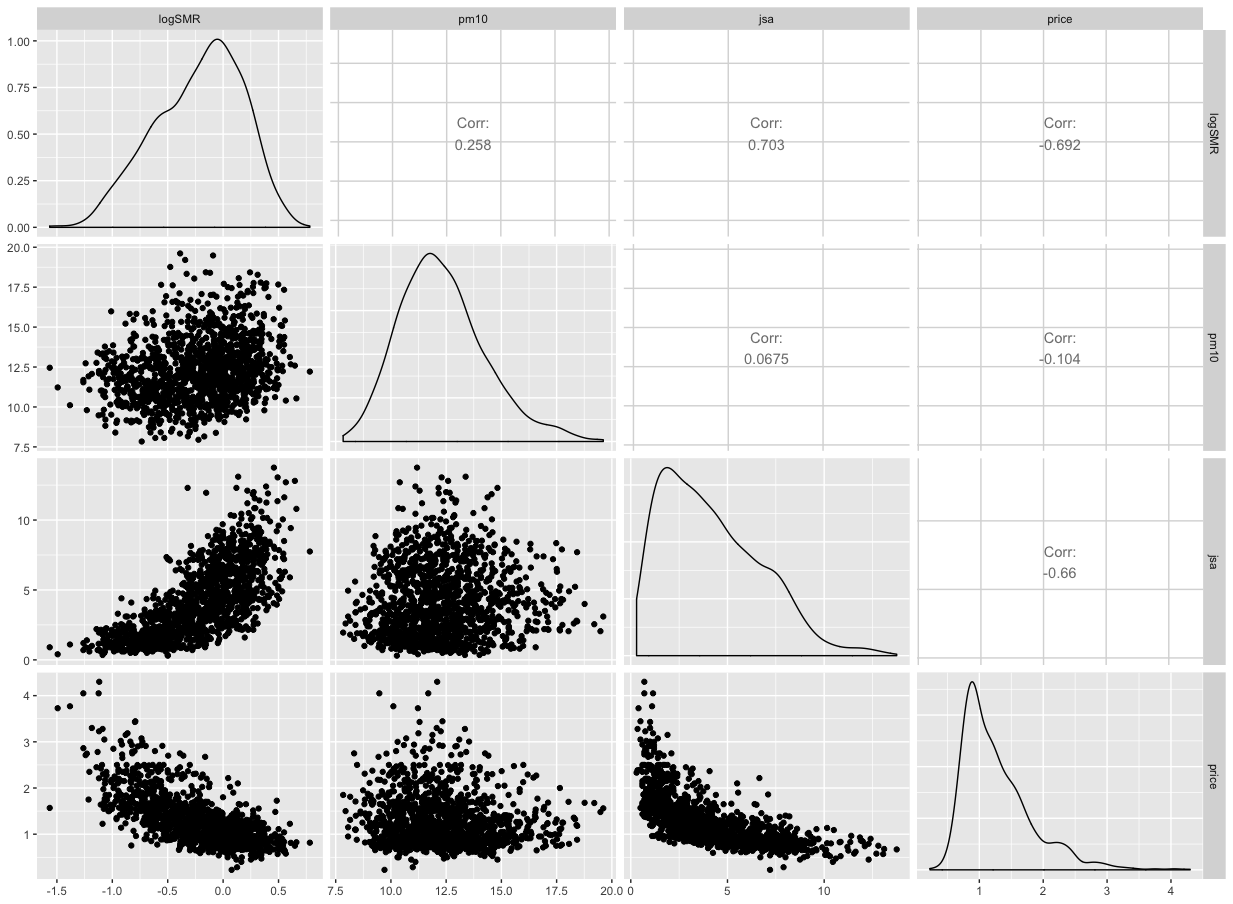
\includegraphics{pollutionscatterplot.png}}
\caption{Scatterplot of the disease, pollution and covariate data.\label{pollution_scatterplot}}
\end{figure} 


The pairs plot shown in Figure \ref{pollution_scatterplot} shows respectively positive and negative relationships between the natural log of SMR and the two deprivation covariates \code{jsa} and \code{price}, in both cases suggesting that increasing levels of poverty are related to an increased risk of respiratory hospitalisation. There also appears to be a weak positive relationship between log(SMR) and PM$_{10}$, while the only relationship that exists between the covariates  is a negative non-linear one between \code{jsa} and \code{price}. Next, it is of interest to visualise the average spatial pattern in the SMR over all five years, and the data can be appropriately aggregated using the \code{summarise()} function from the \pkg{dplyr} package using the code below. The final line adds the aggregated averages to the \code{GGHB.IG} \code{SpatialPolygonsDataFrame} object.


\begin{Schunk}
\begin{Sinput}
R>  group_IG <- group_by(pollutionhealthdata, IG)
R>  SMR.av <- summarise(group_IG, SMR.mean = mean(SMR))
R>  GGHB.IG@data$SMR <- SMR.av$SMR.mean
\end{Sinput}
\end{Schunk}

A spatial map of the aggregated \code{SMR} variable can be overlaid on an OpenStreetMap using the functionality of the \pkg{leaflet} package. However, first the \code{GGHB.IG} object needs to have its coordinate reference system changed to longitude and latitude as this is what the \pkg{leaflet} package requires, which can be done using the following \proglang{R} code.



\begin{Schunk}
\begin{Sinput}
R>  library(rgdal)
R>  GGHB.IG <- spTransform(GGHB.IG, CRS("+proj=longlat +datum=WGS84 +no_defs"))
\end{Sinput}
\end{Schunk}

Then a map of \code{SMR} can be drawn using the following code.

\begin{Schunk}
\begin{Sinput}
R>  library(leaflet)
R>  colours <- colorNumeric(palette = "YlOrRd", domain = GGHB.IG@data$SMR)
R>  map1 <- leaflet(data=GGHB.IG) %>% 
+     addTiles() %>% 
+     addPolygons(fillColor = ~colours(SMR), weight=1, color="",
+                 fillOpacity = 0.7) %>%
+     addLegend(pal = colours, values = GGHB.IG@data$SMR, opacity = 1, 
+                 title="SMR") %>%
+     addScaleBar(position="bottomleft")
R>  map1
\end{Sinput}
\end{Schunk}




\begin{figure}
\centering 
\scalebox{0.8}{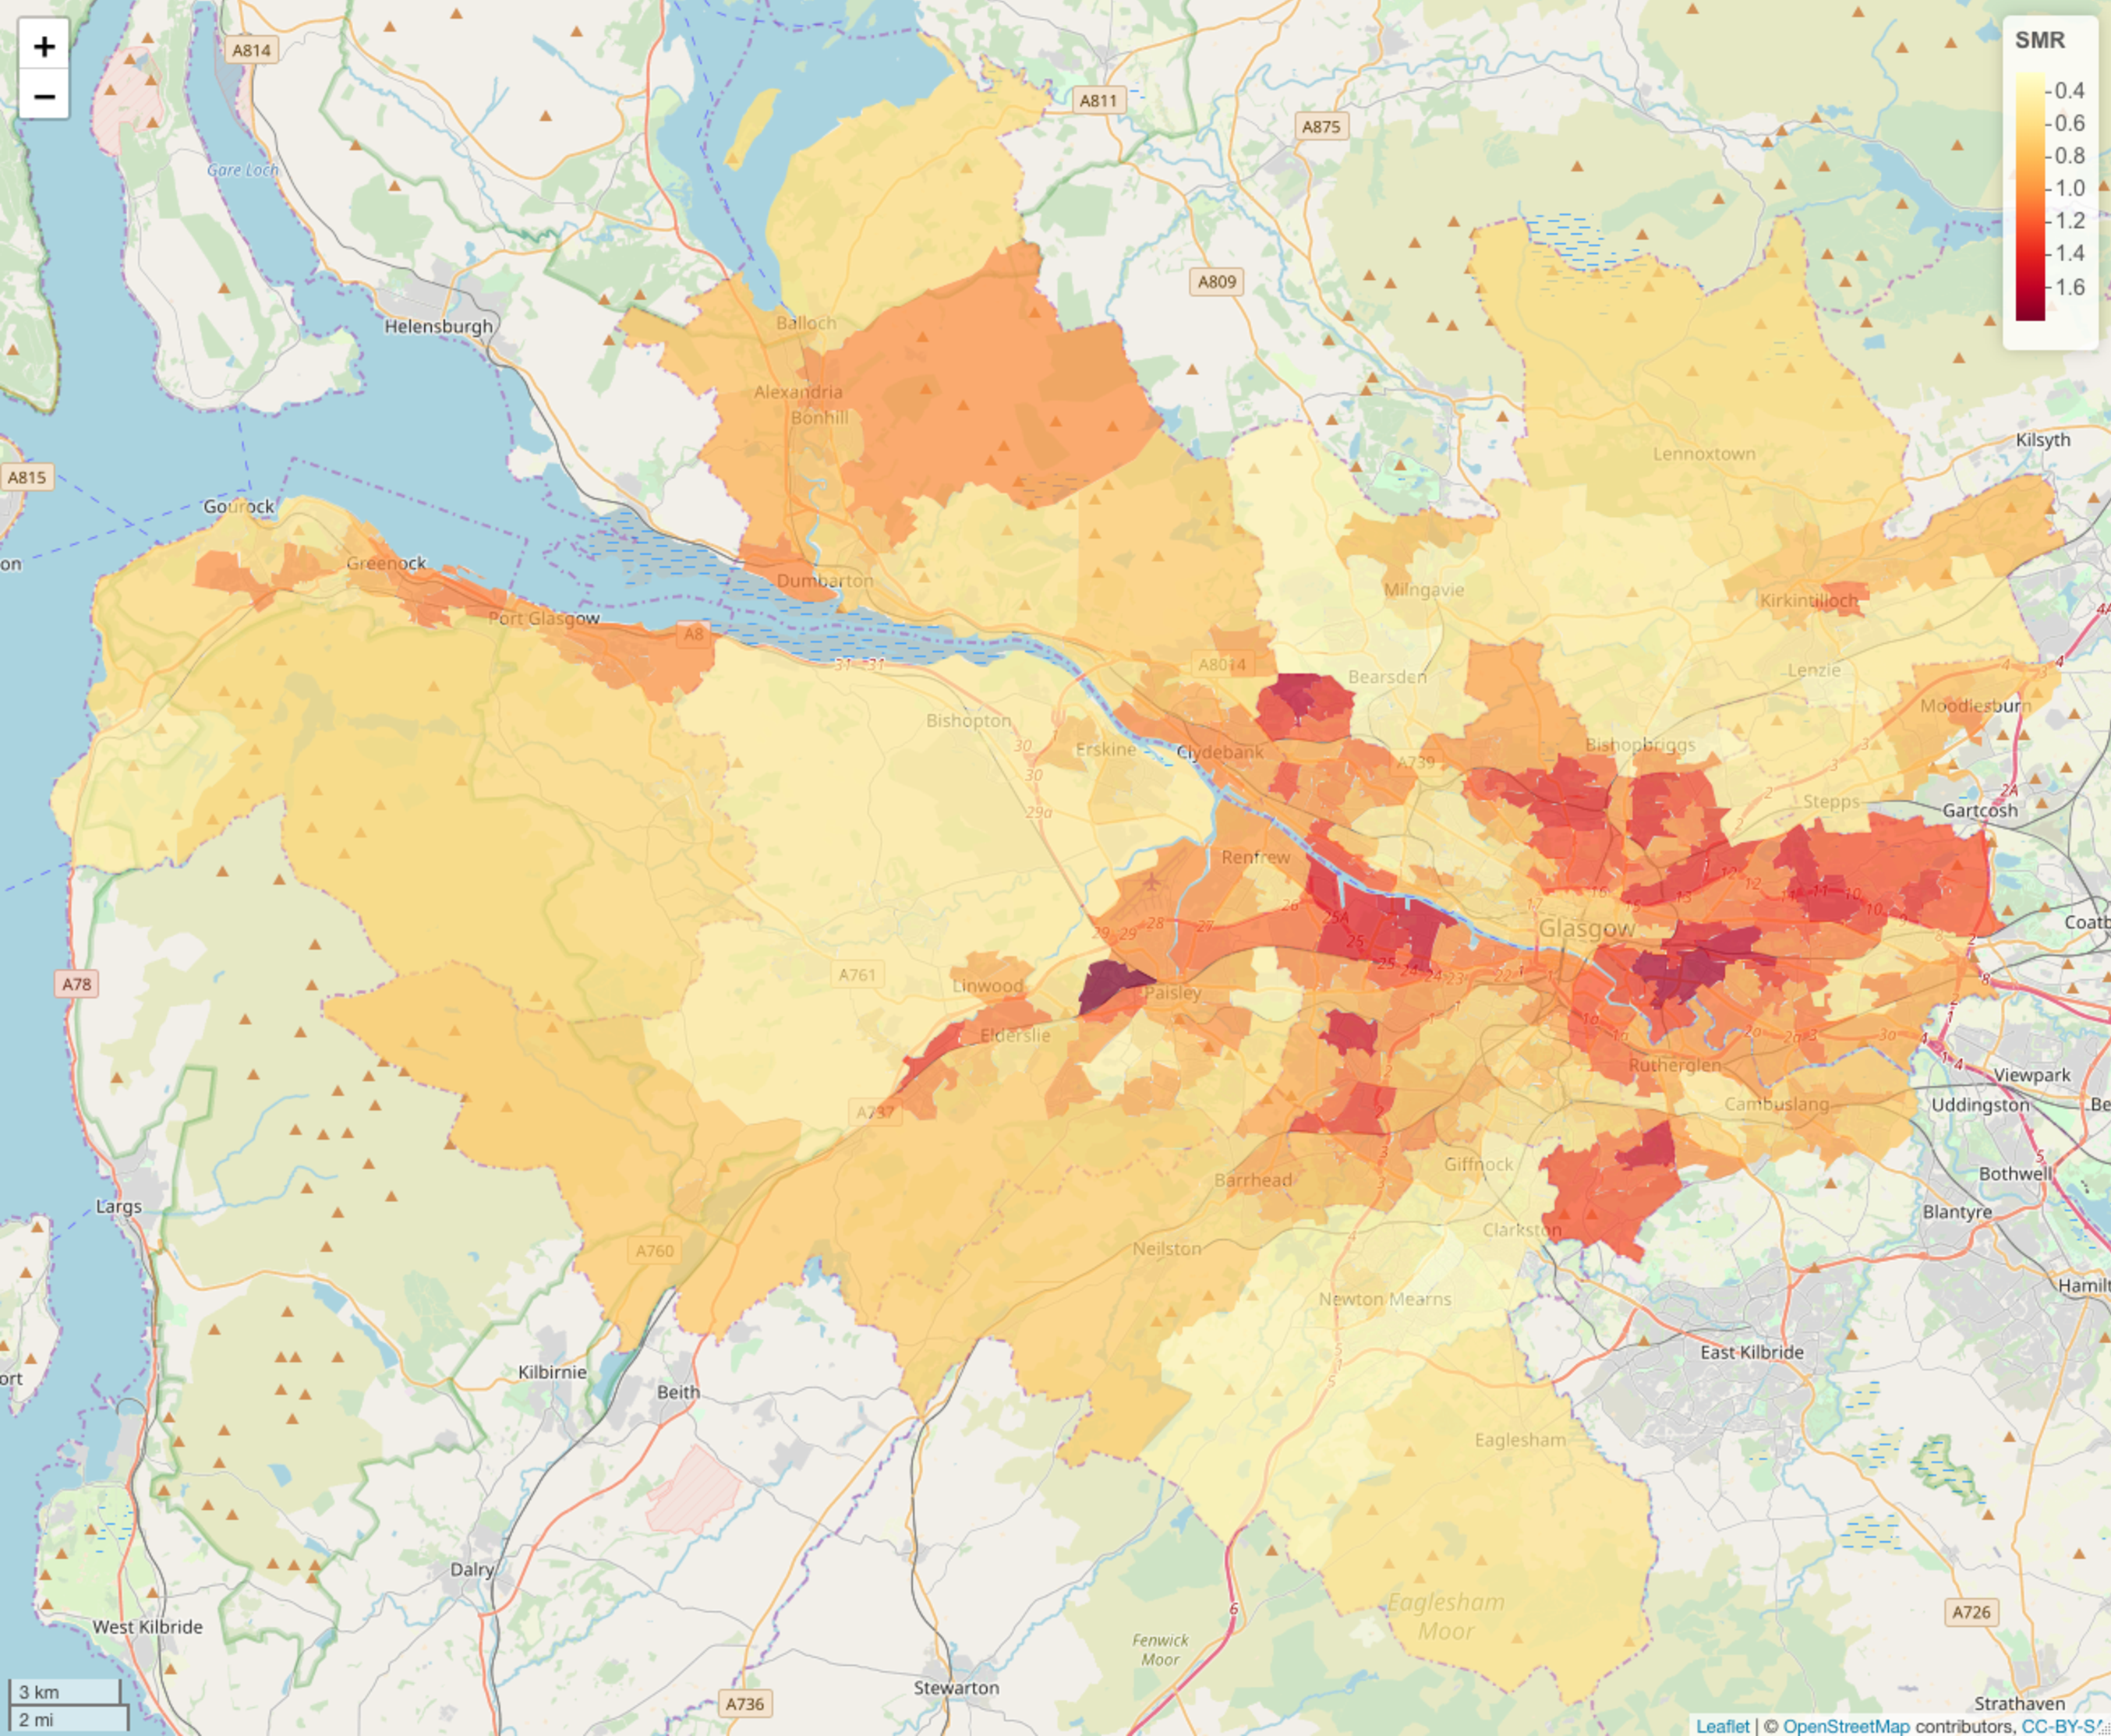
\includegraphics{SMRmap.pdf}}
\caption{Map showing the average SMR over all five years from 2007 to 2011.\label{smr_map}}
\end{figure} 


The map is shown in Figure \ref{smr_map}, where the yellow shaded areas are low risk (SMR$<$1) while the red areas exhibit elevated risks (SMR$>$1). The map shows that the main high-risk areas are in the east-end of Glasgow in the east of the study region, and the Greenock area in the far west of the region on the lower bank of the river Clyde. The spatio-temporal models we fit to these data require the neighbourhood matrix $\mathbf{W}$ and a \code{listw} object variant of the same spatial information, the latter being used in a hypothesis test for spatial autocorrelation. Both of these quantities can be computed from the  \code{SpatialPolygonsDataFrame} object using functionality from the \pkg{spdep} package as follows.

\begin{Schunk}
\begin{Sinput}
R>  library("spdep")
R>  W.nb <- poly2nb(GGHB.IG, row.names = SMR.av$IG)
R>  W.list <- nb2listw(W.nb, style = "B")
R>  W <- nb2mat(W.nb, style = "B")
\end{Sinput}
\end{Schunk}

Here \code{W} is a binary $K\times K$ neighbourhood matrix computed based on sharing a common border, and \code{W.list} is the \code{listw} object variant of this spatial information.


\subsection{Assessing the presence of residua spatial autocorrelation}
The spatio-temporal models in \pkg{CARBayesST} allow for any remaining spatio-temporal autocorrelation in the disease data after the effects of the known covariates have been accounted for. Therefore, we assess the presence of spatial autocorrelation in the residuals from a simple overdispersed Poisson log-linear model that incorporates the covariate effects. This model is fitted using the code:

\begin{Schunk}
\begin{Sinput}
R>  formula <- observed ~ offset(log(expected)) + jsa + price + pm10
R>  model1 <- glm(formula = formula, family = "quasipoisson", 
+     data = pollutionhealthdata)
R>  resid.glm <- residuals(model1)
R>  summary(model1)$coefficients
\end{Sinput}
\begin{Soutput}
               Estimate  Std. Error   t value     Pr(>|t|)
(Intercept) -0.59752496 0.054333524 -10.99735 5.287385e-27
jsa          0.06041994 0.003231475  18.69732 1.467196e-69
price       -0.28293191 0.018292049 -15.46748 8.225472e-50
pm10         0.04174701 0.003282156  12.71938 4.344434e-35
\end{Soutput}
\begin{Sinput}
R>  summary(model1)$dispersion
\end{Sinput}
\begin{Soutput}
[1] 4.399561
\end{Soutput}
\end{Schunk}

The results show significant effects of all three covariates on disease risk, as well as substantial overdispersion with respect to the Poisson equal mean and variance assumption (over dispersion parameter equal to around $4.40$). To quantify the presence of spatial autocorrelation in the residuals from this model we compute Moran's I statistic (\citealp{moran1950}) and conduct a permutation test for each year of data separately. The permutation test has the null hypothesis of no spatial autocorrelation and an alternative hypothesis of positive spatial autocorrelation, and is conducted using the \code{moran.mc()} function from the \pkg{spdep} package. The test can be implemented for the first year of residuals (2007) using the code below.

\begin{Schunk}
\begin{Sinput}
R>  moran.mc(x = resid.glm[1:271], listw = W.list, nsim = 10000)
\end{Sinput}
\begin{Soutput}
	Monte-Carlo simulation of Moran I

data:  resid.glm[1:271] 
weights: W.list  
number of simulations + 1: 10001 

statistic = 0.10358, observed rank = 9967, p-value = 0.0034
alternative hypothesis: greater
\end{Soutput}
\end{Schunk}

The estimated Moran's I statistic is 0.10358 and the p-value is less than 0.05, suggesting strong evidence of unexplained spatial autocorrelation in the residuals from 2007 after accounting for the covariate effects. Similar results were obtained for the other years and are not shown for brevity. We note that residual temporal autocorrelation could be assessed similarly for each IG, for example by computing the lag-1 autocorrelation coefficient, but with only 5 time points the resulting estimates would not be reliable. These results show that the assumption of independence is not valid for these data, and that spatio-temporal autocorrelation should be allowed for when estimating the covariate effects. 


\subsection[Spatio-temporal modelling with CARBayesST]{Spatio-temporal modelling with \pkg{CARBayesST}}
We allow for this residual autocorrelation by applying the \code{ST.CARar()} model with a first order temporal autoregressive structure to the data, details of which are given in Section \ref{section2}. The model can be fitted with the following one-line function call, and we note that all data vectors (response, offset and covariates) have to be ordered so that the first $K$ data points relate to all spatial units at time 1, the next $K$ data points to all spatial units at time 2 and so on. Here we fit the model 3 times which gives results from 3 independent Markov chains.


\begin{CodeInput}
R>  library("CARBayesST")
R>  chain1 <- ST.CARar(formula = formula, family = "poisson", 
+       data = pollutionhealthdata, W = W, burnin = 20000, n.sample = 220000, 
+       thin = 100, AR=1)
R>  chain2 <- ST.CARar(formula = formula, family = "poisson", 
+       data = pollutionhealthdata, W = W, burnin = 20000, n.sample = 220000, 
+       thin = 100, AR=1)
R>  chain3 <- ST.CARar(formula = formula, family = "poisson", 
+       data = pollutionhealthdata, W = W, burnin = 20000, n.sample = 220000, 
+       thin = 100, AR=1)
\end{CodeInput}


In the above code the covariate and offset component defined by \code{formula} is the same as for the simple Poisson log-linear model fitted earlier, and the neighbourhood matrix  \code{W} is also defined above. The \code{ST.CARar}() model is run for three parallel Markov chains, each of which  are run for 220,000 MCMC samples with the first 20,000 samples removed as the burn-in period. The samples are then thinned by 100 to reduce the autocorrelation in the Markov chains, resulting in 6,000 samples for inference. A summary of one of the Markov chain runs can be visualised using the \code{print()} function developed for \pkg{CARBayesST} as shown below.

\begin{CodeInput}
R>  print(chain1)
\end{CodeInput}


\begin{CodeOutput}
#################
#### Model fitted
#################
Likelihood model - Poisson (log link function) 
Latent structure model - Autoregressive CAR model
Regression equation - observed ~ offset(log(expected)) + jsa + price + pm10

############
#### Results
############
Posterior quantities for selected parameters and DIC

             Median    2.5%   97.5% n.effective Geweke.diag
(Intercept) -0.6715 -0.8478 -0.4923       668.8        -1.1
jsa          0.0646  0.0547  0.0753       141.5        -1.7
price       -0.1961 -0.2389 -0.1525      1334.9         1.4
pm10         0.0357  0.0231  0.0469       573.2         1.3
tau2         0.0584  0.0486  0.0686      1766.7        -0.8
rho.S        0.5536  0.3970  0.7133      1761.7        -1.1
rho.T        0.7584  0.6989  0.8174      1995.3        -0.8

DIC =  10400.35       p.d =  773.3225       LMPL =  -5355.437 \end{CodeOutput}


The output from the \code{print()} function is split into two sections, the first part (\code{Model fitted}) describes the model that was fitted, while the second part (\code{Results}) presents  a summary of the numerical results. This summary includes parameter estimates (column \code{Median}), 95\% credible intervals (the columns headed \code{2.5\%} and \code{97.5\%}) and convergence diagnostics (columns \code{n.effective} and \code{Geweke.diag}) for certain parameters, as well as overall model fit measures such as the DIC. The model object \code{chain1} is a list, and details of its elements are described in Section \ref{section3} of this paper. A list object containing the MCMC samples for each individual parameter and the fitted values are stored in \code{chain1$samples}, and each element of this list corresponds to a different group of parameters and is stored as a  \code{mcmc} object from the \pkg{coda} package.  Applying the \code{summary()} function to this object yields:



\begin{CodeInput}
R>  summary(chain1$samples)
\end{CodeInput}




\begin{CodeOutput}
       Length  Class Mode   
beta      8000 mcmc  numeric
phi    2710000 mcmc  numeric
rho       4000 mcmc  numeric
tau2      2000 mcmc  numeric
fitted 2710000 mcmc  numeric
Y            1 mcmc  logical
\end{CodeOutput}



Here the \code{Y} object is \code{NA} as there are no missing $Y_{kt}$ observations in this data set. If there had been say $m$ missing values, then the \code{Y} component of the list would have contained $m$ columns, with each one containing posterior predictive samples for one of the missing observations. Before making inference from the model you have to ensure the Markov chains appear to have converged, and one single chain diagnostic is that proposed by Geweke and given in the model summary above (\code{Geweke.diag}). Another method is a traceplot comparing the results from the multiple chains, which for the regression parameters (\code{beta}) can be produced as follows using functionality from the \pkg{coda} package.

\begin{CodeInput}
R>  library(coda)
R>  beta.samples <- mcmc.list(chain1$samples$beta, chain2$samples$beta, 
+           chain3$samples$beta)
R>  plot(beta.samples)
\end{CodeInput}

The plot is shown in Figure \ref{pollution_mcmc} and superficially shows good mixing between and convergence of the chains, as they all have very similar means and show little trend from left to right. The other commonly used diagnostic is the potential scale reduction factor (PSRF, \cite{gelman2013}), and a value less than 1.1 is suggestive of convergence. The PSRF is computed using the code


\begin{figure}
\centering 
\scalebox{0.8}{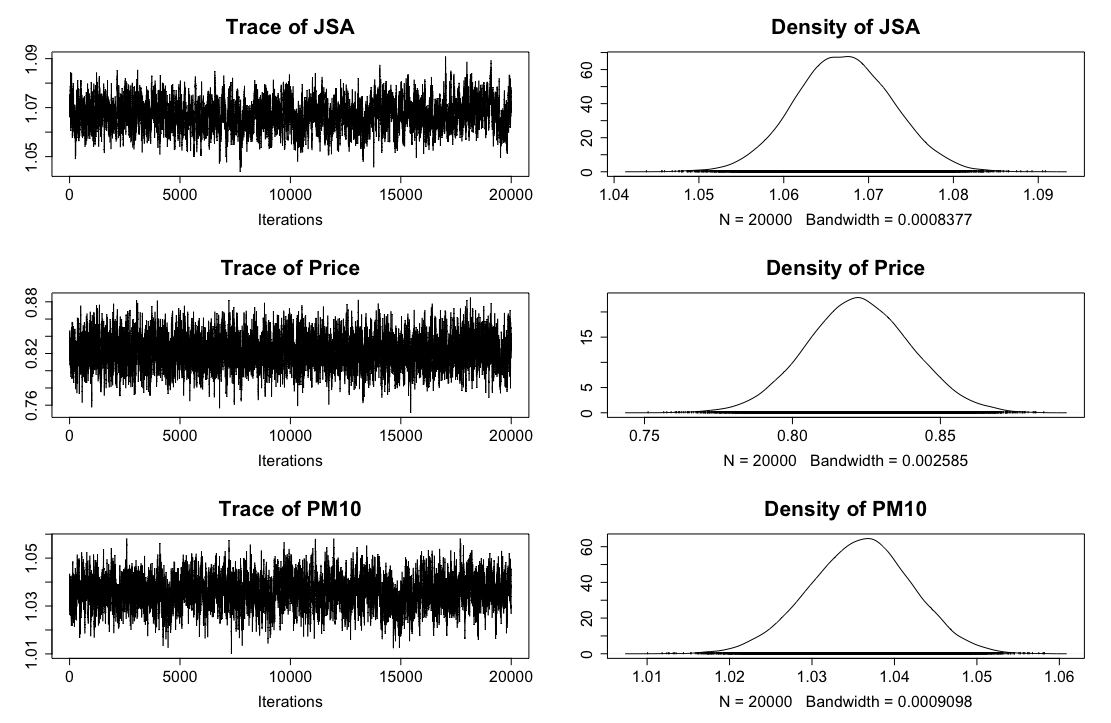
\includegraphics{pollution_mcmc.png}}
\caption{Convergence of the Markov chains.\label{pollution_mcmc}}
\end{figure} 




\begin{CodeInput}
R>  gelman.diag(beta.samples)
\end{CodeInput}


\begin{CodeOutput}
Potential scale reduction factors:

     Point est. Upper C.I.
[1,]       1.00       1.00
[2,]       1.01       1.04
[3,]       1.00       1.02
[4,]       1.00       1.01

Multivariate psrf

1.02
\end{CodeOutput}

which again suggests that the 3 chains are sufficient for making inference. The key interest in this analysis is the effects of the covariates on disease risk, which for Poisson models are typically presented as relative risks. The relative risk for an $\epsilon$ unit increase in a covariate with regression parameter $\beta_s$ is given by the transformation $\exp(\epsilon\beta_s)$, and a relative risk of 1.02 corresponds to a 2\% increased risk if the covariate increased by $\epsilon$. The code below computes the posterior median and 95\% credible intervals  for the relative risks associated with a one unit increase in each covariate, which are all realistic increases given the variation observed in the data in Figure \ref{pollution_scatterplot}.

\begin{CodeInput}
R>  beta.samples <- rbind(chain1$samples$beta[ ,-1], chain2$samples$beta[ ,-1], 
+           chain3$samples$beta[ ,-1])
R>  t(round(apply(exp(beta.samples), 2, quantile, c(0.5, 0.025, 0.975)), 3))
\end{CodeInput}


\begin{CodeOutput}
      50%  2.5% 97.5%
[1,] 1.067 1.056 1.078
[2,] 0.822 0.789 0.859
[3,] 1.036 1.023 1.048
\end{CodeOutput}


The output above shows that the posterior median and 95\% credible interval for the relative risk of a 1$\mu gm^{-3}$  increase in PM$_{10}$ is 1.036 (1.023, 1.048), suggesting that such an increase corresponds to 3.5\% additional hospital admissions. The corresponding relative risk for a one percent increase in JSA is 1.067 (1.056, 1.078), while for a one hundred thousand pounds increase in  property price (the units for the  property price data were in hundreds of thousands) the risk is 0.822 (0.789, 0.859). Thus, we find that increased air pollution concentrations are related, at this ecological level, to increased respiratory hospitalisation, while decreased socio-economic deprivation, as measured by both property price and JSA, is related to decreased risks of hospital admission.





%%%%%%%%%%%%%%
%%%% Section 6
%%%%%%%%%%%%%%
\section{Example 2 - Monitoring the changing state of the housing market}\label{section6}
This second example focuses on the state of the housing market, specifically property sales, and aims to quantify its changing trend over time in an era that encompassed the global financial crisis that began in late 2007. 

\subsection{Data and exploratory analysis}
The study region is the same as for the first example, namely the set of $K=271$ intermediate geographies that make up the Greater Glasgow and Clyde health board. The data also come from the same source (Scottish Statistics, \url{http://statistics.gov.scot/}), and include yearly observations of the number of property sales $Y_{kt}$ in each IG (indexed by $k$) and year (indexed by $t$). Additionally,  we have the total number of properties $n_{kt}$ in each IG and year that will be used in the model as the offset term. We use the following Poisson log-linear model for these data, $Y_{kt}\sim\mbox{Poisson}(n_{kt}\theta_{kt})$, where $\theta_{kt}$ is the rate of property sales as a proportion of the total number of properties. We note that we have not used a binomial model here as a single property could sell more than once in a year, meaning that each property does not constitute a Bernoulli trial. Thus $\theta_{kt}$ is not strictly the proportion of properties that sell in a year, but is on approximately the same scale for interpretation purposes. These data are available in the \pkg{CARBayesdata} package in the object \code{salesdata}, as is the spatial polygon information for the Greater Glasgow and Clyde health board study region (in the object \code{GGHB.IG}). These data can be loaded using the following commands.



\begin{Schunk}
\begin{Sinput}
R>  library("CARBayesdata")
R>  library("sp")
R>  data("GGHB.IG")
R>  data("salesdata")
R>  head(salesdata)
\end{Sinput}
\begin{Soutput}
         IG year sales stock
1 S02000260 2003   122  2002
2 S02000261 2003    54   908
3 S02000262 2003    83  1693
4 S02000263 2003    65  1198
5 S02000264 2003   124  2305
6 S02000265 2003    37  1109
\end{Soutput}
\end{Schunk}


The \code{data.frame} \code{salesdata} contains 4 columns, the intermediate geography code (\code{IG}), the year the data relate to (\code{year}), the number of property sales (\code{sales}, $Y_{kt}$) and the total number of properties (\code{stock}, $n_{kt}$). We visualise the temporal trend in the raw rate of property sales as a proportion of the total number of properties using boxplots via the \pkg{ggplot2} package as shown below.

\begin{Schunk}
\begin{Sinput}
R>  salesdata <- salesdata %>% mutate(salesprop = salesdata$sales / salesdata$stock)
R>  library(ggplot2)
R>  ggplot(salesdata, aes(x = factor(year), y = salesprop)) +
+     geom_boxplot(fill="red", alpha=0.7) + 
+     scale_x_discrete(name = "Year") +
+     scale_y_continuous(name = "Sales proportion") + 
+     theme(text=element_text(size=16), plot.title=element_text(size=18, face="bold")) 
\end{Sinput}
\end{Schunk}


\begin{figure}
\centering 
\scalebox{1}{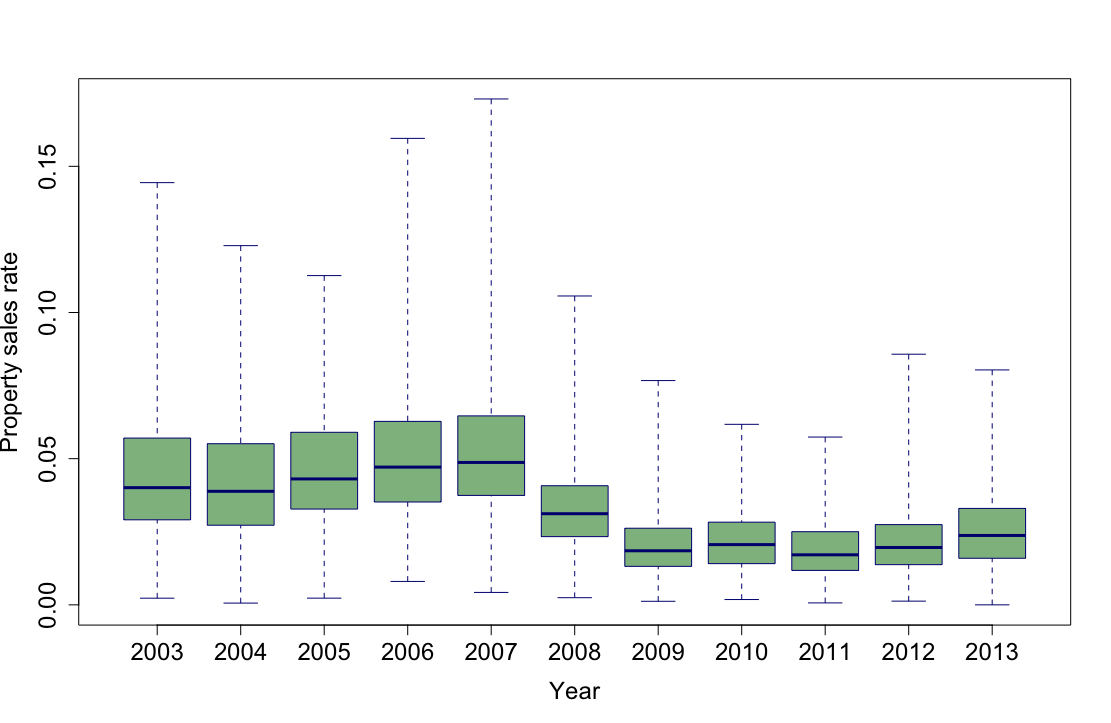
\includegraphics{salesboxplot.png}}
\caption{Boxplots showing the temporal trend in the raw rate of property sales as a proportion of the total number of properties between 2003 and 2013.\label{salesboxplot}}
\end{figure} 


This produces the boxplot shown in Figure \ref{salesboxplot}, where the global financial crisis began in 2007. The plot shows a clear step-change in property sales between 2007 and 2008, as sales were increasing up to and including 2007 before markedly decreasing in subsequent years. Sales in the last year of 2013 show slight evidence of increasing relative to the previous 4 years, possibly suggesting the beginning of an upturn in the market. Also there appears to be a change in the level of spatial variation from year to year, with larger amounts of spatial variation observed before the global financial crisis. The spatial pattern in the average (over time) rate of property sales as a proportion of the total number of properties is computed using the code below.

\begin{Schunk}
\begin{Sinput}
R>  library(dplyr)
R>  group_IG <- group_by(salesdata, IG)
R>  salesprop <- summarise(group_IG, salesproprtion.mean = mean(salesprop))
R>  GGHB.IG@data$sales <- salesprop$salesproprtion.mean
\end{Sinput}
\end{Schunk}

This variable can be mapped using the code below, and the result is displayed in Figure \ref{salesmap}.

\begin{Schunk}
\begin{Sinput}
R>  library(rgdal)
R>  GGHB.IG <- spTransform(GGHB.IG, CRS("+proj=longlat +datum=WGS84 +no_defs"))
R>  library(leaflet)
R>  colours <- colorNumeric(palette = "YlOrRd", domain = GGHB.IG@data$sales)
R>  map1 <- leaflet(data=GGHB.IG) %>% 
+     addTiles() %>% 
+     addPolygons(fillColor = ~colours(sales), color="", weight=1, 
+                 fillOpacity = 0.7) %>%
+     addLegend(pal = colours, values = GGHB.IG@data$sales, opacity = 1, 
+                 title="Sales") %>%
+     addScaleBar(position="bottomleft")
R>  map1
\end{Sinput}
\end{Schunk}



\begin{figure}
\centering 
\scalebox{0.8}{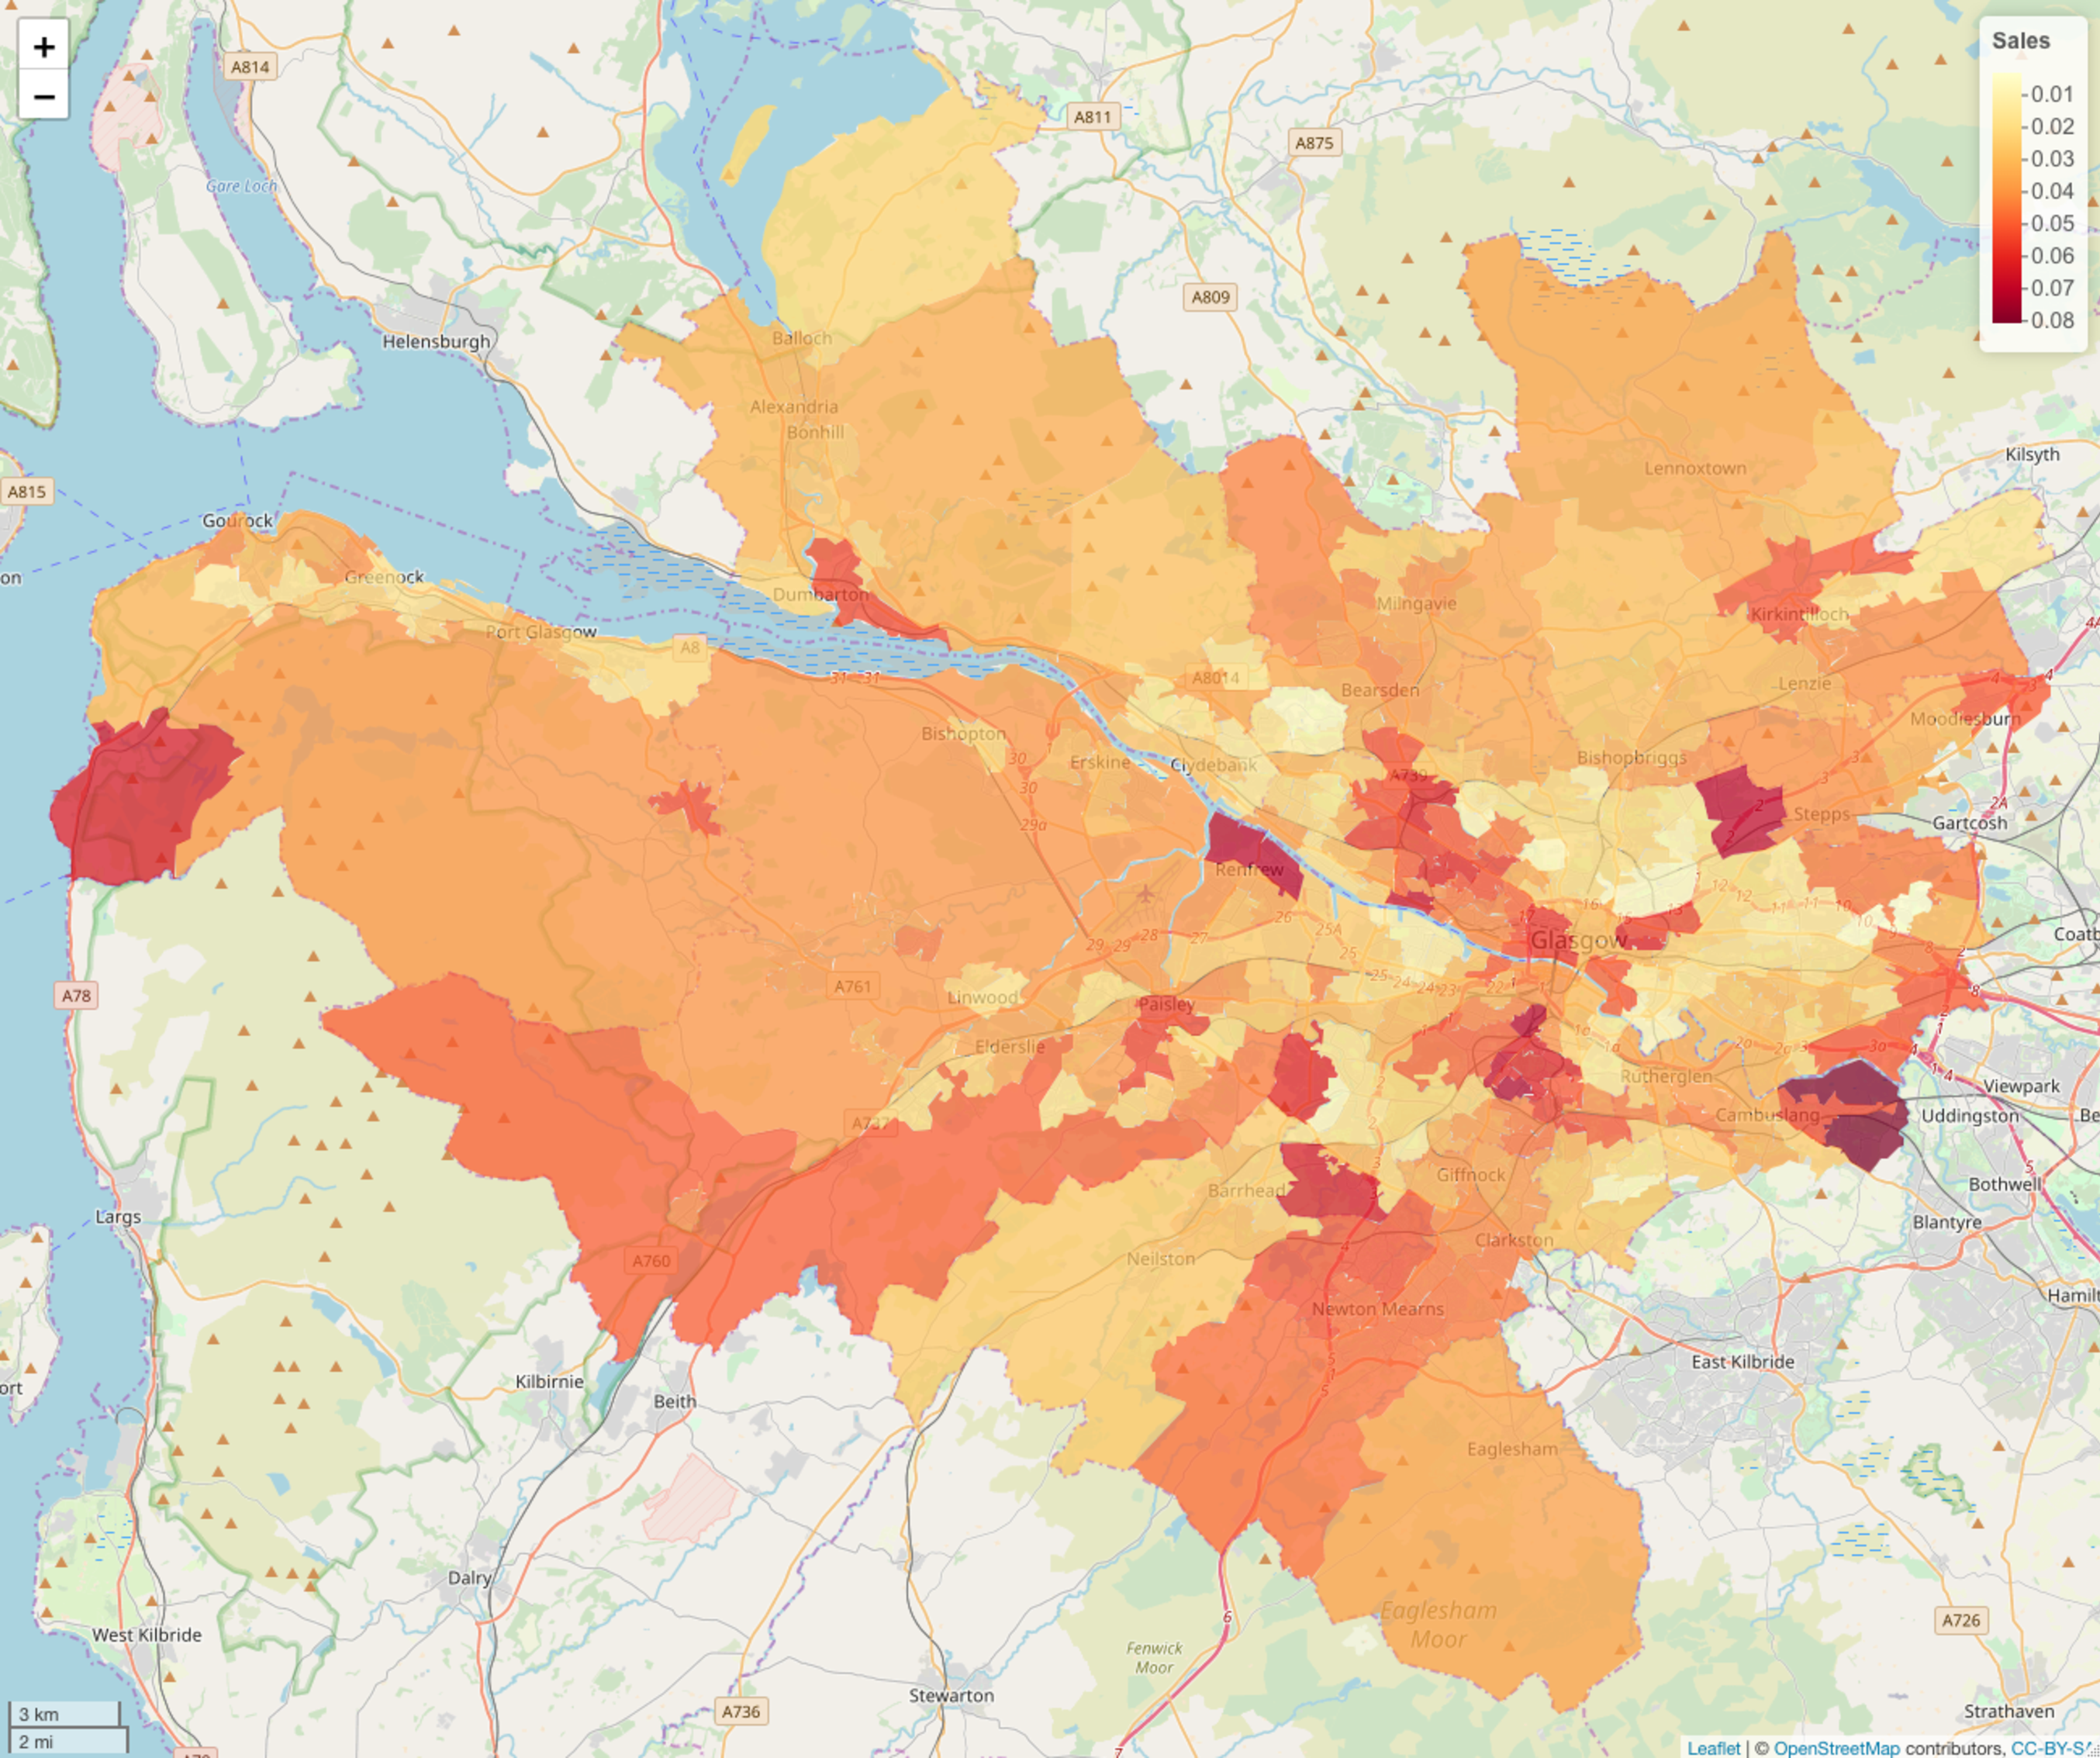
\includegraphics{salesmap.pdf}}
\caption{Map showing the average (between 2003 to 2013) raw rate of property sales as a proportion of the total number of properties.\label{salesmap}}
\end{figure} 


The map shows a largely similar pattern to that seen for respiratory disease risk in Figure \ref{smr_map}, with areas that exhibit relatively high sales rates largely being the same ones that exhibit relatively low disease risk. Figures \ref{salesboxplot} and \ref{salesmap} highlight the change in temporal dynamics and the spatial structure in property sales in Glasgow. Therefore we now apply the \code{ST.CARsepspatial()} model from \pkg{CARBayesST} and proposed by \cite{napier2016}  to more formally quantify these features. This model is chosen because it allows the level of spatial variation to change each year, a feature of the data that is illustrated by Figure \ref{salesboxplot}.

\subsection{Quantifying the changing temporal trends and spatial patterns in sales rates}
Before fitting the model we need to create the neighbourhood matrix using the following code:


\begin{Schunk}
\begin{Sinput}
R>  library("spdep")
R>  W.nb <- poly2nb(GGHB.IG, row.names = salesprop$salesproprtion.mean)
R>  W <- nb2mat(W.nb, style = "B")
\end{Sinput}
\end{Schunk}

Then the model can be fitted using the code below, where inference this time is based on 2,000 post burn-in and thinned MCMC samples from 1 Markov chain. 


\begin{CodeInput}
R>  library("CARBayesST")
R>  formula <- sales ~ offset(log(stock))
R>  chain1 <- ST.CARsepspatial(formula = formula, family = "poisson", 
+           data = salesdata, W = W, burnin = 20000, n.sample = 220000, 
+           thin = 100)
\end{CodeInput}

Convergence of the  Markov chain can be assessed using traceplots and the Geweke diagnostic outlined in the previous section, which are not shown for brevity. Also not shown for brevity is a summary of the fitted model, which as before can be obtained using the \code{print()} function. The model represents the estimated rate of property sales by

$$\theta_{kt}~=~\exp(\beta_1 + \phi_{kt} + \delta_t),$$

which is the sum of an overall intercept term $\beta_1$, a space-time effect $\phi_{kt}$ with a time period specific variance, and a region-wide temporal trend $\delta_t$. The mean and standard deviation of $\{\theta_{kt}\}$ over space for each year is computed by the following code, which produces the posterior median and a 95\% credible interval for each quantity for each year.


\begin{CodeInput}
R>  trend.median <- data.frame(Year=2003:2013, array(NA, c(11, 3)))
R>  colnames(trend.median) <- c("Year", "Median", "LCI", "UCI")
R>  trend.sd <- data.frame(Year=2003:2013, array(NA, c(11, 3)))
R>  colnames(trend.sd) <- c("Year", "Median", "LCI", "UCI")
R>      for(i in 1:11)
+       {
+       posterior <- exp(chain1$samples$phi[ , ((i-1) * 271 + 1):(i * 271)] + 
+                 matrix(rep(chain1$samples$beta + chain1$samples$delta[ , i], 271), 
+                 ncol = 271, byrow = FALSE))
+       trend.median[i, 2:4] <- quantile(apply(posterior, 1, mean), 
+                 c(0.5, 0.025, 0.975))
+       trend.sd[i, 2:4] <- quantile(apply(posterior, 1, sd), 
+                 c(0.5, 0.025, 0.975))
+       }
\end{CodeInput}

The temporal trends in the average rate of property sales and its level of spatial variation can be plotted by the following code, and the result is displayed in Figure \ref{salestrend}.



\begin{CodeInput}
R>  medianplot <- ggplot(aes(x = factor(year), y = salesprop), 
+             data=salesdata) +
+         geom_jitter(color="blue") + 
+         scale_x_discrete(name = "Year") +
+         scale_y_continuous(name = "Average sales rate") + 
+         geom_line(data=trend.median, mapping=aes(x=factor(Year), y=Median, 
+             group=1), colour="red", lwd=1) + 
+         geom_line(data=trend.median, mapping=aes(x=factor(Year), y=LCI, 
+             group=1)) + 
+         geom_line(data=trend.median, mapping=aes(x=factor(Year), y=UCI, 
+             group=1)) + 
+         ggtitle("(a) - Average sales rate") +
+         theme(text=element_text(size=16), plot.title=element_text(size=18, 
+             face="bold")) 

R>  sdplot <- ggplot() +
+         scale_x_discrete(name = "Year") +
+         scale_y_continuous(name = "Spatial standard deviation") + 
+         geom_line(data=trend.sd, mapping=aes(x=factor(Year), y=Median, 
+             group=1), colour="red", lwd=1) + 
+         geom_line(data=trend.sd, mapping=aes(x=factor(Year), y=LCI, 
+             group=1)) + 
+         geom_line(data=trend.sd, mapping=aes(x=factor(Year), y=UCI, 
+             group=1)) + 
+         ggtitle("(b) - Variation in the sales rate") +
+         theme(text=element_text(size=16), plot.title=element_text(size=18, 
+             face="bold")) 

R>  library(gridExtra)
R>  grid.arrange(medianplot, sdplot, nrow=2, ncol=1)
\end{CodeInput}



\begin{figure}
\centering 
\scalebox{1.1}{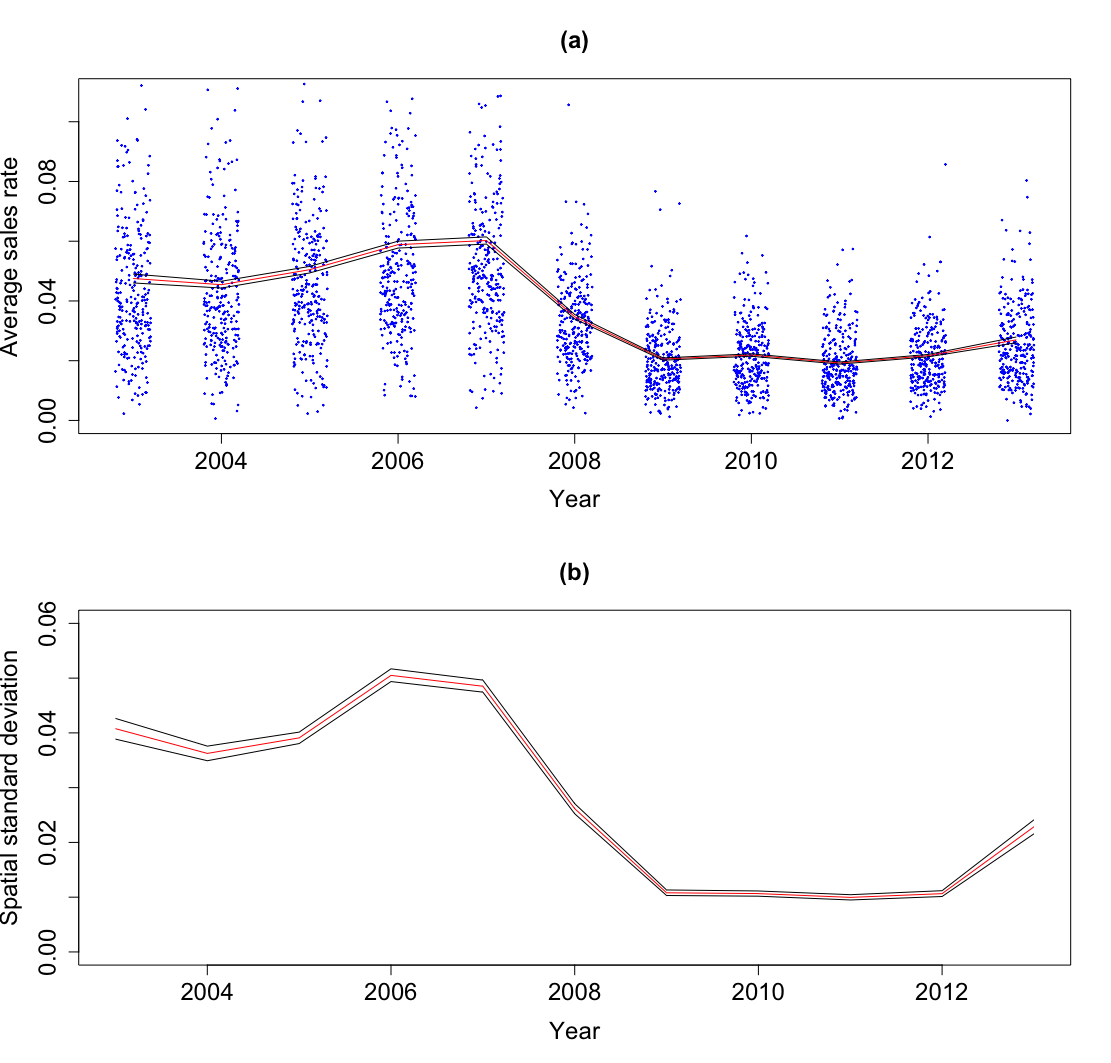
\includegraphics{salestrend.png}}
\caption{Posterior median (red) and 95\% credible interval (black) for the temporal trend in: (a) region-wide average property sales rates; and (b) spatial standard deviation in property sales rates. In panel (a) the blue dots are the raw sales proportions for each area and year (jittered in the x direction to improve the presentation).\label{salestrend}}
\end{figure} 

The figure shows that both the region-wide average (panel (a)) and the level of spatial variation (as measured by the spatial standard deviation, panel (b)) in the rates of property sales show similar underlying trends, with maximum values just before the global financial crisis in 2007, and then  decreases afterwards. This provides some empirical evidence that the global financial crisis negatively affected the housing market in Greater Glasgow, with average sales rates dropping from around 5.0\% (0.05) in 2007 to 3\% (0.03) in 2009. The spatial standard deviation also dropped from 0.045 to 0.01 over the same three-year period, suggesting that the global financial crisis had the effect of reducing the disparity in sales rates in different regions of Greater Glasgow.




%%%%%%%%%%%%%%
%%%% Section 7
%%%%%%%%%%%%%%
\section{Discussion}\label{section7}
\pkg{CARBayesST} is the first software package dedicated to fitting spatio-temporal CAR type models to areal unit data, with inference in a Bayesian setting using MCMC simulation. Future development of the software will focus on extending the number of spatio-temporal models that can be implemented, giving the user an even wider set of modelling tools for both univariate and multivariate spatio-temporal data. 





\section{Acknowledgements}
The Development of \pkg{CARBayesST} was supported by the UK Engineering and Physical Sciences Research Council (EPSRC, grants EP/J017442/1 and EP/T004878/1) and the UK Medical Research Council (MRC, grant MR/L022184/1). The data and shapefiles used in this vignette were provided by the Scottish Government via their Scottish Statistics website (\url{http://statistics.gov.scot/}).


\bibliography{JSS2728}
\end{document}


